\documentclass{article} % For LaTeX2e
\usepackage{iclr2022_conference,times}

% Optional math commands from https://github.com/goodfeli/dlbook_notation.
%%%%% NEW MATH DEFINITIONS %%%%%

\usepackage{amsmath,amsfonts,bm}

% Mark sections of captions for referring to divisions of figures
\newcommand{\figleft}{{\em (Left)}}
\newcommand{\figcenter}{{\em (Center)}}
\newcommand{\figright}{{\em (Right)}}
\newcommand{\figtop}{{\em (Top)}}
\newcommand{\figbottom}{{\em (Bottom)}}
\newcommand{\captiona}{{\em (a)}}
\newcommand{\captionb}{{\em (b)}}
\newcommand{\captionc}{{\em (c)}}
\newcommand{\captiond}{{\em (d)}}

% Highlight a newly defined term
\newcommand{\newterm}[1]{{\bf #1}}


% Figure reference, lower-case.
\def\figref#1{figure~\ref{#1}}
% Figure reference, capital. For start of sentence
\def\Figref#1{Figure~\ref{#1}}
\def\twofigref#1#2{figures \ref{#1} and \ref{#2}}
\def\quadfigref#1#2#3#4{figures \ref{#1}, \ref{#2}, \ref{#3} and \ref{#4}}
% Section reference, lower-case.
\def\secref#1{section~\ref{#1}}
% Section reference, capital.
\def\Secref#1{Section~\ref{#1}}
% Reference to two sections.
\def\twosecrefs#1#2{sections \ref{#1} and \ref{#2}}
% Reference to three sections.
\def\secrefs#1#2#3{sections \ref{#1}, \ref{#2} and \ref{#3}}
% Reference to an equation, lower-case.
\def\eqref#1{equation~\ref{#1}}
% Reference to an equation, upper case
\def\Eqref#1{Equation~\ref{#1}}
% A raw reference to an equation---avoid using if possible
\def\plaineqref#1{\ref{#1}}
% Reference to a chapter, lower-case.
\def\chapref#1{chapter~\ref{#1}}
% Reference to an equation, upper case.
\def\Chapref#1{Chapter~\ref{#1}}
% Reference to a range of chapters
\def\rangechapref#1#2{chapters\ref{#1}--\ref{#2}}
% Reference to an algorithm, lower-case.
\def\algref#1{algorithm~\ref{#1}}
% Reference to an algorithm, upper case.
\def\Algref#1{Algorithm~\ref{#1}}
\def\twoalgref#1#2{algorithms \ref{#1} and \ref{#2}}
\def\Twoalgref#1#2{Algorithms \ref{#1} and \ref{#2}}
% Reference to a part, lower case
\def\partref#1{part~\ref{#1}}
% Reference to a part, upper case
\def\Partref#1{Part~\ref{#1}}
\def\twopartref#1#2{parts \ref{#1} and \ref{#2}}

\def\ceil#1{\lceil #1 \rceil}
\def\floor#1{\lfloor #1 \rfloor}
\def\1{\bm{1}}
\newcommand{\train}{\mathcal{D}}
\newcommand{\valid}{\mathcal{D_{\mathrm{valid}}}}
\newcommand{\test}{\mathcal{D_{\mathrm{test}}}}

\def\eps{{\epsilon}}


% Random variables
\def\reta{{\textnormal{$\eta$}}}
\def\ra{{\textnormal{a}}}
\def\rb{{\textnormal{b}}}
\def\rc{{\textnormal{c}}}
\def\rd{{\textnormal{d}}}
\def\re{{\textnormal{e}}}
\def\rf{{\textnormal{f}}}
\def\rg{{\textnormal{g}}}
\def\rh{{\textnormal{h}}}
\def\ri{{\textnormal{i}}}
\def\rj{{\textnormal{j}}}
\def\rk{{\textnormal{k}}}
\def\rl{{\textnormal{l}}}
% rm is already a command, just don't name any random variables m
\def\rn{{\textnormal{n}}}
\def\ro{{\textnormal{o}}}
\def\rp{{\textnormal{p}}}
\def\rq{{\textnormal{q}}}
\def\rr{{\textnormal{r}}}
\def\rs{{\textnormal{s}}}
\def\rt{{\textnormal{t}}}
\def\ru{{\textnormal{u}}}
\def\rv{{\textnormal{v}}}
\def\rw{{\textnormal{w}}}
\def\rx{{\textnormal{x}}}
\def\ry{{\textnormal{y}}}
\def\rz{{\textnormal{z}}}

% Random vectors
\def\rvepsilon{{\mathbf{\epsilon}}}
\def\rvtheta{{\mathbf{\theta}}}
\def\rva{{\mathbf{a}}}
\def\rvb{{\mathbf{b}}}
\def\rvc{{\mathbf{c}}}
\def\rvd{{\mathbf{d}}}
\def\rve{{\mathbf{e}}}
\def\rvf{{\mathbf{f}}}
\def\rvg{{\mathbf{g}}}
\def\rvh{{\mathbf{h}}}
\def\rvu{{\mathbf{i}}}
\def\rvj{{\mathbf{j}}}
\def\rvk{{\mathbf{k}}}
\def\rvl{{\mathbf{l}}}
\def\rvm{{\mathbf{m}}}
\def\rvn{{\mathbf{n}}}
\def\rvo{{\mathbf{o}}}
\def\rvp{{\mathbf{p}}}
\def\rvq{{\mathbf{q}}}
\def\rvr{{\mathbf{r}}}
\def\rvs{{\mathbf{s}}}
\def\rvt{{\mathbf{t}}}
\def\rvu{{\mathbf{u}}}
\def\rvv{{\mathbf{v}}}
\def\rvw{{\mathbf{w}}}
\def\rvx{{\mathbf{x}}}
\def\rvy{{\mathbf{y}}}
\def\rvz{{\mathbf{z}}}

% Elements of random vectors
\def\erva{{\textnormal{a}}}
\def\ervb{{\textnormal{b}}}
\def\ervc{{\textnormal{c}}}
\def\ervd{{\textnormal{d}}}
\def\erve{{\textnormal{e}}}
\def\ervf{{\textnormal{f}}}
\def\ervg{{\textnormal{g}}}
\def\ervh{{\textnormal{h}}}
\def\ervi{{\textnormal{i}}}
\def\ervj{{\textnormal{j}}}
\def\ervk{{\textnormal{k}}}
\def\ervl{{\textnormal{l}}}
\def\ervm{{\textnormal{m}}}
\def\ervn{{\textnormal{n}}}
\def\ervo{{\textnormal{o}}}
\def\ervp{{\textnormal{p}}}
\def\ervq{{\textnormal{q}}}
\def\ervr{{\textnormal{r}}}
\def\ervs{{\textnormal{s}}}
\def\ervt{{\textnormal{t}}}
\def\ervu{{\textnormal{u}}}
\def\ervv{{\textnormal{v}}}
\def\ervw{{\textnormal{w}}}
\def\ervx{{\textnormal{x}}}
\def\ervy{{\textnormal{y}}}
\def\ervz{{\textnormal{z}}}

% Random matrices
\def\rmA{{\mathbf{A}}}
\def\rmB{{\mathbf{B}}}
\def\rmC{{\mathbf{C}}}
\def\rmD{{\mathbf{D}}}
\def\rmE{{\mathbf{E}}}
\def\rmF{{\mathbf{F}}}
\def\rmG{{\mathbf{G}}}
\def\rmH{{\mathbf{H}}}
\def\rmI{{\mathbf{I}}}
\def\rmJ{{\mathbf{J}}}
\def\rmK{{\mathbf{K}}}
\def\rmL{{\mathbf{L}}}
\def\rmM{{\mathbf{M}}}
\def\rmN{{\mathbf{N}}}
\def\rmO{{\mathbf{O}}}
\def\rmP{{\mathbf{P}}}
\def\rmQ{{\mathbf{Q}}}
\def\rmR{{\mathbf{R}}}
\def\rmS{{\mathbf{S}}}
\def\rmT{{\mathbf{T}}}
\def\rmU{{\mathbf{U}}}
\def\rmV{{\mathbf{V}}}
\def\rmW{{\mathbf{W}}}
\def\rmX{{\mathbf{X}}}
\def\rmY{{\mathbf{Y}}}
\def\rmZ{{\mathbf{Z}}}

% Elements of random matrices
\def\ermA{{\textnormal{A}}}
\def\ermB{{\textnormal{B}}}
\def\ermC{{\textnormal{C}}}
\def\ermD{{\textnormal{D}}}
\def\ermE{{\textnormal{E}}}
\def\ermF{{\textnormal{F}}}
\def\ermG{{\textnormal{G}}}
\def\ermH{{\textnormal{H}}}
\def\ermI{{\textnormal{I}}}
\def\ermJ{{\textnormal{J}}}
\def\ermK{{\textnormal{K}}}
\def\ermL{{\textnormal{L}}}
\def\ermM{{\textnormal{M}}}
\def\ermN{{\textnormal{N}}}
\def\ermO{{\textnormal{O}}}
\def\ermP{{\textnormal{P}}}
\def\ermQ{{\textnormal{Q}}}
\def\ermR{{\textnormal{R}}}
\def\ermS{{\textnormal{S}}}
\def\ermT{{\textnormal{T}}}
\def\ermU{{\textnormal{U}}}
\def\ermV{{\textnormal{V}}}
\def\ermW{{\textnormal{W}}}
\def\ermX{{\textnormal{X}}}
\def\ermY{{\textnormal{Y}}}
\def\ermZ{{\textnormal{Z}}}

% Vectors
\def\vzero{{\bm{0}}}
\def\vone{{\bm{1}}}
\def\vmu{{\bm{\mu}}}
\def\vtheta{{\bm{\theta}}}
\def\va{{\bm{a}}}
\def\vb{{\bm{b}}}
\def\vc{{\bm{c}}}
\def\vd{{\bm{d}}}
\def\ve{{\bm{e}}}
\def\vf{{\bm{f}}}
\def\vg{{\bm{g}}}
\def\vh{{\bm{h}}}
\def\vi{{\bm{i}}}
\def\vj{{\bm{j}}}
\def\vk{{\bm{k}}}
\def\vl{{\bm{l}}}
\def\vm{{\bm{m}}}
\def\vn{{\bm{n}}}
\def\vo{{\bm{o}}}
\def\vp{{\bm{p}}}
\def\vq{{\bm{q}}}
\def\vr{{\bm{r}}}
\def\vs{{\bm{s}}}
\def\vt{{\bm{t}}}
\def\vu{{\bm{u}}}
\def\vv{{\bm{v}}}
\def\vw{{\bm{w}}}
\def\vx{{\bm{x}}}
\def\vy{{\bm{y}}}
\def\vz{{\bm{z}}}

% Elements of vectors
\def\evalpha{{\alpha}}
\def\evbeta{{\beta}}
\def\evepsilon{{\epsilon}}
\def\evlambda{{\lambda}}
\def\evomega{{\omega}}
\def\evmu{{\mu}}
\def\evpsi{{\psi}}
\def\evsigma{{\sigma}}
\def\evtheta{{\theta}}
\def\eva{{a}}
\def\evb{{b}}
\def\evc{{c}}
\def\evd{{d}}
\def\eve{{e}}
\def\evf{{f}}
\def\evg{{g}}
\def\evh{{h}}
\def\evi{{i}}
\def\evj{{j}}
\def\evk{{k}}
\def\evl{{l}}
\def\evm{{m}}
\def\evn{{n}}
\def\evo{{o}}
\def\evp{{p}}
\def\evq{{q}}
\def\evr{{r}}
\def\evs{{s}}
\def\evt{{t}}
\def\evu{{u}}
\def\evv{{v}}
\def\evw{{w}}
\def\evx{{x}}
\def\evy{{y}}
\def\evz{{z}}

% Matrix
\def\mA{{\bm{A}}}
\def\mB{{\bm{B}}}
\def\mC{{\bm{C}}}
\def\mD{{\bm{D}}}
\def\mE{{\bm{E}}}
\def\mF{{\bm{F}}}
\def\mG{{\bm{G}}}
\def\mH{{\bm{H}}}
\def\mI{{\bm{I}}}
\def\mJ{{\bm{J}}}
\def\mK{{\bm{K}}}
\def\mL{{\bm{L}}}
\def\mM{{\bm{M}}}
\def\mN{{\bm{N}}}
\def\mO{{\bm{O}}}
\def\mP{{\bm{P}}}
\def\mQ{{\bm{Q}}}
\def\mR{{\bm{R}}}
\def\mS{{\bm{S}}}
\def\mT{{\bm{T}}}
\def\mU{{\bm{U}}}
\def\mV{{\bm{V}}}
\def\mW{{\bm{W}}}
\def\mX{{\bm{X}}}
\def\mY{{\bm{Y}}}
\def\mZ{{\bm{Z}}}
\def\mBeta{{\bm{\beta}}}
\def\mPhi{{\bm{\Phi}}}
\def\mLambda{{\bm{\Lambda}}}
\def\mSigma{{\bm{\Sigma}}}

% Tensor
\DeclareMathAlphabet{\mathsfit}{\encodingdefault}{\sfdefault}{m}{sl}
\SetMathAlphabet{\mathsfit}{bold}{\encodingdefault}{\sfdefault}{bx}{n}
\newcommand{\tens}[1]{\bm{\mathsfit{#1}}}
\def\tA{{\tens{A}}}
\def\tB{{\tens{B}}}
\def\tC{{\tens{C}}}
\def\tD{{\tens{D}}}
\def\tE{{\tens{E}}}
\def\tF{{\tens{F}}}
\def\tG{{\tens{G}}}
\def\tH{{\tens{H}}}
\def\tI{{\tens{I}}}
\def\tJ{{\tens{J}}}
\def\tK{{\tens{K}}}
\def\tL{{\tens{L}}}
\def\tM{{\tens{M}}}
\def\tN{{\tens{N}}}
\def\tO{{\tens{O}}}
\def\tP{{\tens{P}}}
\def\tQ{{\tens{Q}}}
\def\tR{{\tens{R}}}
\def\tS{{\tens{S}}}
\def\tT{{\tens{T}}}
\def\tU{{\tens{U}}}
\def\tV{{\tens{V}}}
\def\tW{{\tens{W}}}
\def\tX{{\tens{X}}}
\def\tY{{\tens{Y}}}
\def\tZ{{\tens{Z}}}


% Graph
\def\gA{{\mathcal{A}}}
\def\gB{{\mathcal{B}}}
\def\gC{{\mathcal{C}}}
\def\gD{{\mathcal{D}}}
\def\gE{{\mathcal{E}}}
\def\gF{{\mathcal{F}}}
\def\gG{{\mathcal{G}}}
\def\gH{{\mathcal{H}}}
\def\gI{{\mathcal{I}}}
\def\gJ{{\mathcal{J}}}
\def\gK{{\mathcal{K}}}
\def\gL{{\mathcal{L}}}
\def\gM{{\mathcal{M}}}
\def\gN{{\mathcal{N}}}
\def\gO{{\mathcal{O}}}
\def\gP{{\mathcal{P}}}
\def\gQ{{\mathcal{Q}}}
\def\gR{{\mathcal{R}}}
\def\gS{{\mathcal{S}}}
\def\gT{{\mathcal{T}}}
\def\gU{{\mathcal{U}}}
\def\gV{{\mathcal{V}}}
\def\gW{{\mathcal{W}}}
\def\gX{{\mathcal{X}}}
\def\gY{{\mathcal{Y}}}
\def\gZ{{\mathcal{Z}}}

% Sets
\def\sA{{\mathbb{A}}}
\def\sB{{\mathbb{B}}}
\def\sC{{\mathbb{C}}}
\def\sD{{\mathbb{D}}}
% Don't use a set called E, because this would be the same as our symbol
% for expectation.
\def\sF{{\mathbb{F}}}
\def\sG{{\mathbb{G}}}
\def\sH{{\mathbb{H}}}
\def\sI{{\mathbb{I}}}
\def\sJ{{\mathbb{J}}}
\def\sK{{\mathbb{K}}}
\def\sL{{\mathbb{L}}}
\def\sM{{\mathbb{M}}}
\def\sN{{\mathbb{N}}}
\def\sO{{\mathbb{O}}}
\def\sP{{\mathbb{P}}}
\def\sQ{{\mathbb{Q}}}
\def\sR{{\mathbb{R}}}
\def\sS{{\mathbb{S}}}
\def\sT{{\mathbb{T}}}
\def\sU{{\mathbb{U}}}
\def\sV{{\mathbb{V}}}
\def\sW{{\mathbb{W}}}
\def\sX{{\mathbb{X}}}
\def\sY{{\mathbb{Y}}}
\def\sZ{{\mathbb{Z}}}

% Entries of a matrix
\def\emLambda{{\Lambda}}
\def\emA{{A}}
\def\emB{{B}}
\def\emC{{C}}
\def\emD{{D}}
\def\emE{{E}}
\def\emF{{F}}
\def\emG{{G}}
\def\emH{{H}}
\def\emI{{I}}
\def\emJ{{J}}
\def\emK{{K}}
\def\emL{{L}}
\def\emM{{M}}
\def\emN{{N}}
\def\emO{{O}}
\def\emP{{P}}
\def\emQ{{Q}}
\def\emR{{R}}
\def\emS{{S}}
\def\emT{{T}}
\def\emU{{U}}
\def\emV{{V}}
\def\emW{{W}}
\def\emX{{X}}
\def\emY{{Y}}
\def\emZ{{Z}}
\def\emSigma{{\Sigma}}

% entries of a tensor
% Same font as tensor, without \bm wrapper
\newcommand{\etens}[1]{\mathsfit{#1}}
\def\etLambda{{\etens{\Lambda}}}
\def\etA{{\etens{A}}}
\def\etB{{\etens{B}}}
\def\etC{{\etens{C}}}
\def\etD{{\etens{D}}}
\def\etE{{\etens{E}}}
\def\etF{{\etens{F}}}
\def\etG{{\etens{G}}}
\def\etH{{\etens{H}}}
\def\etI{{\etens{I}}}
\def\etJ{{\etens{J}}}
\def\etK{{\etens{K}}}
\def\etL{{\etens{L}}}
\def\etM{{\etens{M}}}
\def\etN{{\etens{N}}}
\def\etO{{\etens{O}}}
\def\etP{{\etens{P}}}
\def\etQ{{\etens{Q}}}
\def\etR{{\etens{R}}}
\def\etS{{\etens{S}}}
\def\etT{{\etens{T}}}
\def\etU{{\etens{U}}}
\def\etV{{\etens{V}}}
\def\etW{{\etens{W}}}
\def\etX{{\etens{X}}}
\def\etY{{\etens{Y}}}
\def\etZ{{\etens{Z}}}

% The true underlying data generating distribution
\newcommand{\pdata}{p_{\rm{data}}}
% The empirical distribution defined by the training set
\newcommand{\ptrain}{\hat{p}_{\rm{data}}}
\newcommand{\Ptrain}{\hat{P}_{\rm{data}}}
% The model distribution
\newcommand{\pmodel}{p_{\rm{model}}}
\newcommand{\Pmodel}{P_{\rm{model}}}
\newcommand{\ptildemodel}{\tilde{p}_{\rm{model}}}
% Stochastic autoencoder distributions
\newcommand{\pencode}{p_{\rm{encoder}}}
\newcommand{\pdecode}{p_{\rm{decoder}}}
\newcommand{\precons}{p_{\rm{reconstruct}}}

\newcommand{\laplace}{\mathrm{Laplace}} % Laplace distribution

\newcommand{\E}{\mathbb{E}}
\newcommand{\Ls}{\mathcal{L}}
\newcommand{\R}{\mathbb{R}}
\newcommand{\emp}{\tilde{p}}
\newcommand{\lr}{\alpha}
\newcommand{\reg}{\lambda}
\newcommand{\rect}{\mathrm{rectifier}}
\newcommand{\softmax}{\mathrm{softmax}}
\newcommand{\sigmoid}{\sigma}
\newcommand{\softplus}{\zeta}
\newcommand{\KL}{D_{\mathrm{KL}}}
\newcommand{\Var}{\mathrm{Var}}
\newcommand{\standarderror}{\mathrm{SE}}
\newcommand{\Cov}{\mathrm{Cov}}
% Wolfram Mathworld says $L^2$ is for function spaces and $\ell^2$ is for vectors
% But then they seem to use $L^2$ for vectors throughout the site, and so does
% wikipedia.
\newcommand{\normlzero}{L^0}
\newcommand{\normlone}{L^1}
\newcommand{\normltwo}{L^2}
\newcommand{\normlp}{L^p}
\newcommand{\normmax}{L^\infty}

\newcommand{\parents}{Pa} % See usage in notation.tex. Chosen to match Daphne's book.

\DeclareMathOperator*{\argmax}{arg\,max}
\DeclareMathOperator*{\argmin}{arg\,min}

\DeclareMathOperator{\sign}{sign}
\DeclareMathOperator{\Tr}{Tr}
\let\ab\allowbreak


\usepackage{hyperref}
\usepackage{url}
\usepackage{amssymb}
\usepackage{graphicx}
\iclrfinalcopy
%\setlength{\tabcolsep}{10pt}
%\renewcommand{\arraystretch}{1.5}

\title{HERMES : Hybrid ERror-corrector Model with inclusion of External Signals for nonstationary fashion time series}

\author{Etienne DAVID \\
Heuritech \\
Paris \\
\texttt{etienne.david@heuritech.com} \\
\And
Sylvain Le Corff \\
Samovar, T\'el\'ecom SudParis, d\'epartement CITI, TIPIC \\
Institut Polytechnique de Paris, Palaiseau \\
\texttt{sylvain.le$\_$corff@telecom-sudparis.eu} \\
\And 
Jean Bellot \\
Heuritech \\
Paris \\
\texttt{jean.bellot@heuritech.com} \\
}

% The \author macro works with any number of authors. There are two commands
% used to separate the names and addresses of multiple authors: \And and \AND.
%
% Using \And between authors leaves it to \LaTeX{} to determine where to break
% the lines. Using \AND forces a linebreak at that point. So, if \LaTeX{}
% puts 3 of 4 authors names on the first line, and the last on the second
% line, try using \AND instead of \And before the third author name.

\newcommand{\fix}{\marginpar{FIX}}
\newcommand{\new}{\marginpar{NEW}}

\newcommand{\ts}{y}
\newcommand{\fullts}{{\bf \ts}}
\newcommand{\tspred}{\hat{\ts}}
\newcommand{\stat}{f}
\newcommand{\statparam}{\theta_{predictor}}
\newcommand{\fullstat}{{\bf \stat}}
\newcommand{\lag}{h}
\newcommand{\window}{w}
\newcommand{\tswindow}{{\bf \ts}}
\newcommand{\meants}{\Bar{\ts}}
\newcommand{\rnnwindow}{{\bf \rnninput}}
\newcommand{\rnninput}{z}
\newcommand{\rnn}{\textsc{rnn}}
\newcommand{\rnnparam}{\theta_{corrector}}
\newcommand{\err}{err}
\newcommand{\errwindow}{{\bf \err}}
\newcommand{\rnnmodel}{\textsc{rnn}}
\newcommand{\ws}{w}
\newcommand{\fullws}{{\bf \ws}}
\newcommand{\wswindow}{{\bf \ws}}
\newcommand{\concatinput}{x}
\newcommand{\fullconcatinput}{{ \bf \concatinput}}
\newcommand{\numberts}{10000}
\newcommand{\threshold}{\eta}
\newcommand{\predictor}{\mathrm{RNN}_p}
\newcommand{\classifier}{\mathrm{RNN}_c}
\newcommand{\remainder}{r}
\newcommand{\hiddenregime}{U}


%\iclrfinalcopy % Uncomment for camera-ready version, but NOT for submission.
\begin{document}


\maketitle

\begin{abstract}
Developing models and algorithms to draw causal inference for time series is a long standing statistical problem. It is crucial for many applications, in particular for fashion or retail industries, to make optimal inventory decisions and avoid massive wastes. By tracking thousands of fashion trends on social media with state-of-the-art computer vision approaches, we propose a new model for fashion time series forecasting. Our contribution is  twofold. We first provide the first fashion dataset gathering \numberts\ weekly fashion time series. As influence dynamics are the key of emerging trend detection, we associate with each time series several external weak signals representing behaviors of influencers towards the trend. Secondly, to leverage such a complex and rich dataset, we propose a new hybrid forecasting model. Our approach combines per-time-series parametric models with seasonal components and a global recurrent neural network to include sporadic external signals. This hybrid model provides state-of-the-art results on the fashion dataset, and illustrates the benefit of the contribution of external weak signals.
\end{abstract}

\section{Introduction}

Multivariate time series forecasting is a widespread statistical problem with  many applications, see for instance \citep{sarkka2013bayesian, douc2014nonlinear, zucchini2017hidden} and the numerous references therein.
 %Due to the diversity of applications and use cases, a multitude of models have been proposed. 
 Parametric generative models allow to provide explainable predictions with statistical guarantees based on a precise modeling of the predictive distributions of new data based on a record of past observations. %The parameters of these models are usually estimated using a sequence of observations of the target time series. 
Calibrating these models, for instance using maximum likelihood inference, often requires a fair amount of tuning to design a time series-specific model to provide  accurate forecasts and sharp confidence intervals.  Depending on the use case, statistical properties of the signal and the available data, many families of models have been proposed for time series.  The exponential smoothing model \citep{RePEc:inm:oropre:v:9:y:1961:i:5:p:673-685}, the Trigonometric Box-Cox transform, ARMA errors, Trend, and Seasonal components model (TBATS) \cite{doi:10.1198/jasa.2011.tm09771}, or the ARIMA with the Box-Jenkins approach \citep{box2015time} are for instance very popular parametric linear generative models.  Hidden Markov models (HMM) are also widespread and presuppose that available observations are defined using missing data describing the dynamical system. This hidden state is assumed to be a Markov chain such that at each time step the received observation is a random function of the corresponding latent data.  Although hidden states are modeled as a Markov chain, the observations arising therefrom present a highly complex statistical structure. %Introducing latent hidden states, they assume that the predictive distribution is not unique and constant in time but multiple and lead by the values of the hidden states changing during time. 
 In various applications where signals exhibit non-stationarities such as trends and seasonality, classical HMM are not adapted. However, \citep{touron2017modeling}  recently proposed seasonal HMM, assuming that transition probabilities between the states, as well as the emission distributions, are not constant in time but evolve in a periodic manner. Strong consistency results were established in \citep{touron2019consistency} and Expectation Maximization based numerical experiments were proposed.
Altough these works provide promising results, HMM are computationally expensive to train and are not yet well studied for seasonal  sequences with thousands of components.
 
 %However, for a large part of applications, parametric generative approaches show limitation to capture  complexity. Accurate candidates can be found with latent data models.  

%During the past decades, forecasting applications have taken a totally new proportion. 
In many fields, single or few time series have become thousands of sequences with complex statistical structures. In this new context, classical time series specific statistical models show limitations when dealing with numerous heterogeneous data. Recurrent neural networks and recent sequence to sequence deep learning architectures offer very appealing numerical alternatives thanks to their capability of leveraging any kind of heterogeneous multivariate data, see for instance \citep{ hochreiter1997long,vaswani2017attention, 8614252, li2019enhancing, lim2019temporal,salinas2020deepar}. %In the past decades, with the impressive results of deep neural networks (DNN) in vision or language, some time series forecasting applications have been proposed. 
%Significant improvements have been achieved with Reccurent Neural Network and its Long Short-Term Memory (LSTM) or Gated Recurrent Unit (GRU)  declinations \citep{}. 
The DeepAR model proposed in \citep{salinas2020deepar} provides a global model from many time series based on
a multi-layer recurrent neural network with LSTM cells. More recently, applications using the Transformer model have been proposed  \citep{li2019enhancing}. A direct concurrent of the DeepAR model can be found with the Temporal Fusion Transformers (TFT) approach \citep{lim2019temporal}.  Unfortunately, all these solutions suffer from two main weaknesses. Firstly, many of them are "black-boxes"  as the final forecast usually does not come with a statistical guarantee  although a few recent works focused on measuring uncertainty in recurrent neural networks, see  \cite{martin2020monte}. Secondly, without a fine prepossessing and well chosen hyper-parameters, these methods may lead to poor results and are often outperformed by traditional statistical models, see \cite{makridakis2018m4}.

In this paper, we consider  new time series forecasting application referred to as {\em fashion trends prediction}. Based on a cutting-edge image recognition technology, we built the first fashion dataset containing \numberts\ sequences representing the apparition of fashion trends on social media per week from 01-01-2015 to 01-01-2019. Our fashion time series has very appealing properties: they have all the same length, same seasonality, no missing value and the absence of sparse time series even for niche trends. The originality of our dataset come from the fact that additional external weak signals can be introduced. With our fashion expertise, we detected several groups of fashion users with a high influence power. Analysing their specific behaviours on social medias, we add to each time series, 4 external weak signals representing the same fashion trends but on a sub-category of users. We call them weak signals because they are often alerts or events that are too sparse, or too incomplete to allow on their own an accurate estimation of their impact on the prediction of the target signal. With this totally new application, we aim at designing a model able to deal with our large fashion dataset, leverage our complex external weak signals and finally provide the most accurate forecasts.
 
Recurrent neural networks are appealing to tackle our forecasting problem due to their capability of leveraging external data.  Recently, hybrid models combining deep neural network (DNN) architectures with widespread statistical models to deal with seasonality and trends have been proposed, see for instance  \citep{zhang2003time,jianwei2019novel,bandara2020lstm}. The approach providing the most striking results was proposed in  \citep{smyl2020hybrid} in the context of the M4 forecasting competition \citep{makridakis2020m4}.  Given a large dataset, a per-time-series multiplicative exponential smoothing model is introduced to estimate simple but fundamental components for each time series and compute a first prediction. Then a global recurrent neural network is trained on the entire dataset to correct errors of the previous exponential smoothing models. %With this process, the hybrid approach succeeds at mixing strengths of both model families: robustness of the time series specific parametric models and the power of neural network at learn complex dynamics on large dataset. 
%However, the hybrid model has not been designed to deal with external signals even if it include a neural network.

%Following this work, we present in this paper a new hyrbid recurrent model for time series forecasting with inclusion of external weak signals. %We design a more general hybrid framework including the original multiplicative model and a new additive one. 
%Our approach enriches existing hybrid models by incorporating an unobserved regime switching feature to account for the need of a neural network based correction. In order to leverage external signals, we modify the hybrid framework to allow the regime shift and the  global error-corrector neural network to deal with external data.

Following this work, we present in this paper HERMES, a new hybrid recurrent model for time series forecasting with inclusion of external signals. Our model is decomposed  into two parts: local predictors and a global corrector.  First, a per-time-series parametric statistical model is trained on all sequences. Then,  a global recurrent neural network is trained to evaluate and correct the forecast weaknesses of the first collection of models. By adding external weak signals in our proposed framework, we show the real potential of the hybrid approach: a global neural network, able to leverage large amount of heterogeneous data, deal with any kind of external weak signals, learn context and finally correct weaknesses and errors of any parametric models.
%Our new hybrid framework is divided in two parts. As a first step, we compute a per-time-series forecast for each trend using any kind of parametric models. Then, gathering information of the first prediction and external variables, a global error corrector neural network is trained to correct weaknesses of the first forecast. 


%Section~\ref{sec:hybrid} describes our hybrid framework which consists of a per-time-series parametric model and a recurrent neural network combining the target sequences with external weak signals

The paper is organized as follow. Section~\ref{sec:hybrid} describes our hybrid framework. Then, we present our new fashion dataset in Section~\ref{sec:dataset}. Section~\ref{sec:exp} describes our results and comparisons with several benchmarks. Finally, we detail research perspectives and conclude our paper in Section~\ref{sec:discussion} and Section~\ref{sec:conclusion}.


\section{Hybrid model with external signals}
\label{sec:hybrid}
%We introduce a new hybrid approach for time series forecasting  composed of two parts: a first per time series parametric model with seasonal component and a global RNN. We use a per time series statistical model to learn local behaviour and to normalize sequences before feeding them to the neural network.
%We introduce a new hybrid approach for time series forecasting  composed of two parts: a first per time series parametric model with seasonal component and a global neural network framework composed of two RNN. We use a per time series statistical model to learn local behaviour, to normalize sequences by removing trends and seasonality,  and to compute a first forecast. Then, we use two recurrent neural networks and weak signals to correct, if needed, the predictions provided by the first collection of parametric models.
We introduce a new hybrid approach for time series forecasting  composed of two parts: a collection of per-time-series parametric models, the predictors, and a global error-corrector neural network train on all time series, the corrector. We use  per-time-series parametric models to learn local behaviour, to normalize sequences by removing trends and seasonality,  and to compute a first forecast. Then, gathering information of the first predictions and external variables, we use a recurrent neural networks to correct the predictions provided by the first collection of per-time-series models.

Consider $N\geqslant 1$ time series. For all $1\leqslant n \leqslant N$ and $1\leqslant t \leqslant T$, let $\ts_t^n$ be the value of the $n$-th sequence at time $t$ and  $\fullts^n = \{\ts_t^n\}_{1\leqslant t \leqslant T}$ be all the values of this sequence.   The objective of this paper is to propose a model to  forecast all time series in a given time frame  $\lag \in \mathbb{N}$, i.e. we aim at sampling $\{\ts^n_{T+1:T+\lag}\}_{1\leqslant n \leqslant N}$ based on $\{\ts^n_{1:T}\}_{1\leqslant n \leqslant N}$.

%It is assumed that for all $1\leqslant n \leqslant N$, $\fullts^n$ is a seasonal time series with a season equal to $m \in \mathbb{N}$, $m$ equals 4 for quarterly, 12 for monthly or 52 for weekly time series. However, no restriction in term of scale and noise distributions are assumed in the generative law of each time series.

\subsection{Per-time-series predictors}
%The first step in our additive hybrid model is to consider, for each time series, an exponential smoothing  statistical model.
%The time-series-specific models compute, for each sequence, two components,  level  and  seasonality. For all $1\leqslant n \leqslant N$ and $0\leqslant t \leqslant T$, let $\lvl_t^n$ be the value of the $n$-th level component at time $t$ and  $\fulllvl^n = \{\lvl_t^n\}_{0\leqslant t \leqslant T}$ be all the values of this level component. For all $1\leqslant n \leqslant N$ and $-m+1\leqslant t \leqslant T$, let $\seas_t^n$ be the value of the $n$-th seasonality component at time $t$ and  $\fullseas^n = \{\seas_t^n\}_{-m+1\leqslant t \leqslant T}$ be all the values of this season component. $m \in \mathbb{N}$ is the seasonality (4 for quarterly, 12 for monthly or 52 for weekly time series).
The time-series-specific predictors compute, for each sequence, a first $\lag$-ahead prediction based on the past. For all $1\leqslant n \leqslant N$, we note $\stat^n(.;\statparam^n)$ the $n$-th parametric model of the $n$-th sequence where $\statparam^n$ are  unknown parameters. Given the sequences $\{\ts^n_{1:T}\}_{1\leqslant n \leqslant N}$ and the estimated  parameters $\{\statparam^n\}_{1\leqslant n \leqslant N}$, the time-series-specific forecasts $\{\tspred^{pred,n}_{T+1:T+\lag|T}\}_{1\leqslant n \leqslant N}$ are, for all $n \in \{1,\ldots,N\}$, for all $i \in \{1,\ldots,\lag\}$,
$$
\tspred^{pred,n}_{T+i|T} = \stat^n(\ts^n_{1:T};\statparam^n)_i\,.
$$

During the M4 competition, the hybrid model of \cite{smyl2020hybrid} was based on a multiplicative exponential smoothing model as the time-series-specific predictor. However, on sporadic time series, this choice leads to poor result and instability. In this paper, we provide a general framework able to deal with any kind of per-time-series models. In Section~\ref{sec:exp}, we present two versions of our framework. The first one use an  exponential smoothing as reference similar to the baseline \cite{smyl2020hybrid} and the second one use a TBATS model \cite{doi:10.1198/jasa.2011.tm09771} which provides better results as this parametric model includes  Fourier representations with time varying coefficients, and ARMA error correction. %The main complexity is in the next stage: training a global RNN corrector to improve the per-time-series statistical models when the parametric models start showing weaknesses.

In the specific application of fashion trends prediction, we detected and defined two main forms of standard weaknesses for a univariate parametric forecast as defined above. The first one is a weakness of definition, when the model is not well defined for its forecasting task. For instance, an additive model provide good predictions on time series with additive seasonality but show difficulties with multiplicative one. The second form, harder to detect and correct, is the weakness of information. For non stationary time series, huge changes of behaviours are not always predictable using the past of the sequence. In somes cases, these changes depend on external variables not considered by univariate parametric models. The difficulty is that we mainly unknow the exact influence of external variables on the main signal. It is on this point that our new hybrid framework shows its true potential: introduce a global RNN trained on all the time series and able to consider and leverage external signals.

\medskip

\textcolor{red}{Ajouter ici une figure avec une ou deux series temporelles mal predites par le modele statistique et bien corrigees par le RNN pour illustrer le potentiel.}
% Indeed, depending on time series, some family of parametric models can achieve really heterogeneous level of accuracy. 
%For all $1\leqslant n \leqslant N$, let $\Theta^n = \{\alpha^n, \gamma^n, \lvl^n_0, \{\seas_t^n\}_{-m+1\leqslant t \leqslant 0}\}$ be the parameters of the $n$-th sequence with $\lsmooth^n$ and $\ssmooth^n$ the positive smoothing parameters, $\lvl^n_0$ the first level term and $\{\seas_t^n\}_{-m+1\leqslant t \leqslant 0}$ the $m$ first seasonality terms. Given the sequence $\fullts^n$ and the parameters $\Theta^n$ , the two components  $\fulllvl^n$ and $\fullseas^n$ are computed as follow :
%We initialize the first level with $\lvl^n_{0} = \sum_{t = 1}^m \ts^n_{t}/m$ \textcolor{red}{issue with the time index ?} and, for all $1\leqslant n \leqslant N$ and $1\leqslant t \leqslant T$,
%\begin{align*}
    %\lvl^n_{t} &= \lsmooth^n (\ts^n_t - \seas^n_{t-m}) + (1- \lsmooth^n)\lvl^n_{t-1}\,, \\
    %\seas^n_t &= \ssmooth^n (\ts^n_t - \lvl^n_{t-1}) + (1 - \ssmooth^n)\seas^n_{t-1}\,. 
%\end{align*}

%For all $1\leqslant n \leqslant N$, given the level component $\fulllvl^n$, the seasonality component $\fullseas^n$ and the forecast horizon $\lag \in \mathbb{N}$, the exponential smoothing forecast $\{\etspred^{ets,n}_{T+1:T+\lag|T}\}_{1\leqslant n \leqslant N}$ is, for all $i \in \{1,\ldots,\lag\}$,
%$$
%\etspred^{ets,n}_{T+i|T} = \lvl^n_T + \seas^n_{T+i-m(k+1)}\,,
%$$
%where $k = \lfloor(i-1)/m\rfloor$. 

%For this first stage, we decided to use an additive exponential smoothing for many reasons: firstly, it is easily understandable and it is pretty robust for any kind of sequences. 

%This statistical model offers a fine approach to normalize and deseasonnalize the sequences. In addition, with its two recurrent equations only, it is simple to code and incorporate in a larger framework using deep learning model and GPUs. However, other statistical methods could have been used as the basis of our hybrid approach. For example, S. Smyl created his hybrid model with a multiplicative exponential smoothing model instead of the additive form. At the end, The main complexity is in the next stage: succeed in training a global RNN to understand all the per-time-series statistical models and correct their mistakes.

\subsection{Error-corrector recurrent model}

The second part of our model is a global RNN, trained on all the $N$ sequences to correct the weaknesses of the first per-time-series parametric models. This task requires a thorough data pre-processing for two main reasons. First, we provide  to the RNN the best input in order to understand the initial collection of forecasts and predict their future errors. Second, as we did not make any assumption about the scale of our time series, we have to carefully normalize them before feeding them to the RNN.
Consider the following pre-processing. 
%At this stage, we can write that for all $n \in \{1,\ldots,N\}$, for all $i \in \{1,\ldots,\lag\}$,
%$$
%\ts^n_{T+i} = \tspred^{stat,n}_{T+i|T} + \varepsilon^n_{T+i}\,,
%$$
%In this paper, we introduce a model based on a latent regime. In regime 0, the first parametric forecast succeeds at catching all the information of the $n$-th sequence and the final forecast of our framework is the prediction of the per-time-series parametric model. Conversely, in regime 1, the first parametric forecast is unaccurate and it remains a residual random error term that can be estimated. % quantity that we note $\remainder$. 
%Conditionally on $\{\fullts^n\}_{1\leqslant n\leqslant N}$, our regime-switching model is:

%$$
%\ts^n_{T+i} = \tspred^{stat,n}_{T+i|T} + \hiddenregime^n_T \cdot \remainder^{n}_{T+i} + \varepsilon^n_{T+i} = \stat^n_{\statparam^n}(\ts^n_{1:T})_i + \hiddenregime^n_T \cdot \remainder^{n}_{T+i} + \varepsilon^n_{T+i}\,,
%$$
%where $\{\varepsilon^n_{T+i}\}_{1\leqslant i\leqslant \lag}$ are independent random variables, $U^n_T$ is an unobserved regime switching Bernoulli random variable and $\{\remainder^n_{T+i}\}_{1\leqslant i\leqslant \lag}$ is the random error term to be estimated.
%In the regime 1, the first parametric forecast is unaccurate and it remains a non-forecasted quantity that we note $\remainder$.
%For this regime, we have for all $i \in \{1,\ldots,\lag\}$ :
%$$
%\ts^n_{T+i} = \tspred^{stat,n}_{T+i|T} + \remainder^{n}_{T+i} + \varepsilon^n_{T+i}\,,
%$$

%To estimate this model, we introduce our new regime swithing error-corrector framework. We train two global RNN on all sequences, a classifier ($\classifier$) and a predictor ($\predictor$). We train the classifier to estimate the law of the Bernoulli random variable $\hiddenregime^n_T$ and we train the predictor to predict $\{\remainder^{n}_{T+i}\}_{1\leqslant i\leqslant \lag}$. However, these two tasks require a thorough data pre-processing and with our collection of parametric models, we propose first to normalize and deseasonalize the RNNs inputs.

%Then, we train a global RNN on all sequences to compute a correction of the initial prediction.
%Then, we train a global RNN on all sequences to compute a correction of the initial prediction. %We motivate this choice for two reasons. Firstly, pure machine learning methods achieve relatively poor results in time series forecasting. Turning a full forecasting task into a correcting task largely simplifies the RNN goals. 
%This task requires a thorough data pre-processing and with our collection of parametric models, we propose a fine way to normalize and deseasonalize the RNN inputs and outputs. %We describe bellow how we design a RNN able to understand the first exponential smoothing models and estimate a correction of their forecasting errors.

Let $\window \in \mathbb{N}$ be the window size, usually this window is proportional to the forecast horizon $\window \propto \lag$. We define as our RNN input the following  normalized, deseasonalized and rescaled sequence $\rnnwindow^n_T = \{\rnninput^{n}_{T-\window+i|T}\}_{1\leqslant i \leqslant w}$, where, for all $1\leqslant n \leqslant N$ and $1\leqslant i \leqslant w$, 
$$
\rnninput^{n,T}_{T-w+i|T} = \frac{\ts^n_{T-w+i} -\tspred^{pred,n}_{T+i|T}}{\meants^n_T}\,,\quad\mbox{where}\quad \meants^n_T = \frac{1}{w}\sum_{i = 1}^{w}\ts^n_{T-w+i}\,.
$$


We note $\rnn(.;\rnnparam)$ the recurrent neural network model where $\rnnparam$ are  unknown parameters. Given the RNN input sequences $\{\rnnwindow^n_T\}_{1\leqslant n \leqslant N}$ and the global RNN estimated parameters $\rnnparam$, the error-corrector predictions $\{\tspred^{corr,n}_{T+1:T+\lag|T}\}_{1\leqslant n \leqslant N}$ are, for all $n \in \{1,\ldots,N\}$, for all $i \in \{1,\ldots,\lag\}$,
$$
\tspred^{corr,n}_{T+i|T} = \rnn(\rnnwindow^n_T;\rnnparam)_i \cdot \meants^n_T\ \,.
$$

Our hybrid model forecast is finally given, for all $1\leqslant n \leqslant N$ and all $i \in \{1,\ldots,\lag\}$, by:

\begin{equation}
\label{eq:nows:full:model}
\tspred^n_{T+i|T}  = \tspred^{pred,n}_{T+i|T} +  \tspred^{corr,n}_{T+i|T} = \stat^n(\ts^n_{1:T};\statparam^n)_i +  \rnn(\rnnwindow^n_T;\rnnparam)_i \cdot \meants^n_T\
\end{equation}



%We use this sequence as input of  $\classifier$ and $\predictor$. %Write, for all $1\leqslant n \leqslant N$ and all $i \in \{1,\ldots,H\}$, $\err^{n,T}_{T+i|T} = \ts^n_{T+i} - \etspred^{ets,n}_{T+i|T}$.
% Given $\rnnwindow^n_T$, the proposed regime swithing error-corrector reccurent model is given, for all $1\leqslant n \leqslant N$ and all $i \in \{1,\ldots,\lag\}$, by :
%\begin{align*}
%\ts^n_{T+i}  &= \tspred^{stat,n}_{T-w+i|T} +  \hat{\hiddenregime}^n_T \cdot \hat{\remainder}^{n}_{T+i} + \varepsilon^n_{T+i}\,, \\
%\hat{\hiddenregime}^n_T &= \mathbf{1}_{\classifier(\rnnwindow^n_T) > \threshold}\,, \\
%\hat{\remainder}^{n}_{T+i} &= \predictor(\rnnwindow^n_T)_{T+i} \cdot \meants^n_T\,.
%\end{align*}




%where $\mathbf{1}$ is the indicator function and $\threshold$ a threshold parameter.

%Consider then a recurrent neural network denoted by RNN-p which aims at predicting the exponential smoothing error. Given $\rnnwindow^n_T$, the proposed model is given, for all $1\leqslant n \leqslant N$ and all $i \in \{1,\ldots,\lag\}$, by
%$$
%\ts^n_{T+i}  = \tspred^{stat,n}_{T-w+i|T-w} +  U^n_T\times\meants^n_T\times \rnnmodel_p(\rnnwindow^n_T)_{T+i} + \varepsilon^n_{T+i}\,,%\\
%  &= \stat^n(\ts^n_{1:T}|\statparam^n)_i +  U^n_T\times\meants^n_T\times \rnnmodel_p(\rnnwindow^n_T)_{T+i} + \varepsilon^n_{T+i}\,,
%$$
%where $\{\varepsilon^n_{T+i}\}_{i\leqslant 1}$ are independent random variables with a Laplace distribution and $U^n_T$ an unobserved regime switching Bernoulli random variable. The random variable $U^n_T$ allows to provide RNN-p corrections only when ETS prediction is not sharp enough \textcolor{red}{Show in appendix cases where ETS alone is enough and cases where correction is required}. The law of $U^n_T$ is parameterized by a recurrent neural network denoted by RNN-c with the same input than RNN-p.
%\begin{align*}
%U^n_T = \mathbf{1}_{\rnnmodel_p(\rnnwindow^n_T) > \threshold}
%\end{align*}
%$$
%\ts^n_{T+i} = \rnnmodel(\rnnwindow^n_T)_{T+i} = \frac{\hat{\err}^{n,T}_{T+i|T}}{\meants^n_T}
%$$
%Finally, for all $1\leqslant n \leqslant N$, the  final forecast of the model is $\{\tspred^{n}_{T+1:T+\lag|T}\}_{1\leqslant n \leqslant N}$, where, for all $i \in \{1,\ldots,\lag\}$ :
%\begin{align*}
%\tspred^n_{T+i|T}  &= \etspred^{ets,n}_{T+i|T} +  \meants^n_T\times \rnnmodel(\rnnwindow^n_T)_{T+i}\,,\\
%  &= \lvl^n_T + \seas^n_{T+i-m(k+1)} + \hat{\err}^{n,T}_{T+i|T}\,.
%\end{align*}

\subsection{Weak signal}

Using well-fitted time-series-specific parametric models, our hybrid network corrects the first form of weakness and achieves striking accuracy on our dataset, \textcolor{red}{see Table~XXX}. Then, to correct the second form of weakness, in addition to the $N$ target time series, we consider $K \times N$ external sequences indexed from $0$ to $T$. For all $1\leqslant n \leqslant N$, $1\leqslant k \leqslant K$ and  $1\leqslant t \leqslant T$, let $\ws^{n,k}_t$ be the value of the $k$-th external sequence at time $t$ linked to the sequence $\fullts^n$. We note $\fullws^n = \{\{\ws_t^{n,k}\}_{1\leqslant t \leqslant T}\}_{1\leqslant k \leqslant K}$ all the values of the family of weak signals linked to the $n$-th sequence. In addition, let $\fullws^n_T = \{\{\ws_{T-w+i}^{n,k}\}_{1\leqslant i \leqslant \window}\}_{1\leqslant k \leqslant K}$ be only the last $\window$ terms of the family. Concatenating $ \rnnwindow^n_T$ and $\fullws^n_T$, we define a new input for our RNN,   
$$
\fullconcatinput^n_T = \{\concatinput^n_{T-w+i|T}\}_{1\leqslant i \leqslant w}= \{\rnninput^n_{T-w+i|T}, \ws^{n,1}_{T-w+i},...,\ws^{n,K}_{T-w+i}\}_{1\leqslant i \leqslant w}\,.
$$
Finally, for all $1\leqslant n \leqslant N$ and for all $i \in \{1,\ldots,\lag\}$ our final model becomes:
%$$
%\tspred^n_{T+i|T} 
%= \etspred^{ets,n}_{T+i|T} +  \rnnmodel(\fullconcatinput^n_T)_{T+i} \times \meants^n_T
%$$
\begin{equation}
\label{eq:withws:full:model}
\tspred^n_{T+i|T}  = \tspred^{pred,n}_{T+i|T} +  \tspred^{corr,n}_{T+i|T} = \stat^n(\ts^n_{1:T};\statparam^n)_i +  \rnn(\fullconcatinput^n_T;\rnnparam)_i \cdot \meants^n_T\
\end{equation}

An illustration of our proposed architecture is displayed in Figure~\ref{fig:architecture}.

\begin{figure}
  \centering
    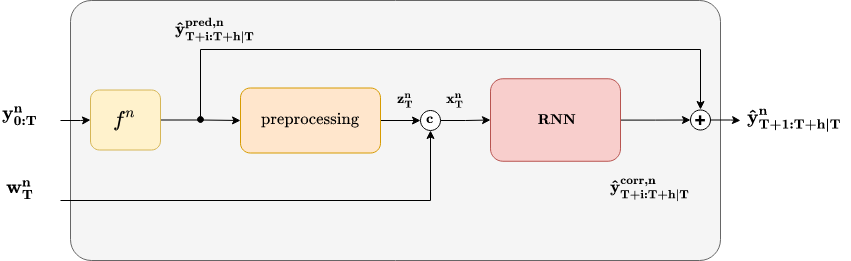
\includegraphics[width=1\linewidth]{figure/HERMES_archi.png}
  \caption{Hybrid model with weak signals architecture.}
\label{fig:architecture}
\end{figure}


%\subsection{Hidden regime}

%As the regime is not observed, the loglikelihood of the observations cannot be written explicitly to train the model. Therefore we use Fisher's identity to compute the score function and write a gradient ascent algorithm to estimate simultaneously the weights of RNN-p and of RNN-c denoted by $\rnnparam = \{\rnnparam_c,\rnnparam_p\}$. The score is
%\begin{equation}
%\label{eq:score}
%\nabla_\theta \log p_\theta(\ts^n_{T+1:T+h}|\ts^n_{1:T}) = \mathbb{E}\left[\nabla_\theta \log p_\theta(\ts^n_{T+1:T+h},U_T^n|\ts^n_{1:T})\middle|\ts^n_{1:T+h}\right]\,,
%\end{equation}
%where the joint likelihood $p_\theta(\ts^n_{T+1:T+h},U_T^n|\ts^n_{1:T}) = p_\theta(U_T^n|\ts^n_{1:T})p_\theta(\ts^n_{T+1:T+h}|U_T^n,\ts^n_{1:T})$ is given by \eqref{eq:full:model} and the expectation is under the posterior distribution of $U_T^n$ given $\ts^n_{1:T+h}$. Write $\omega_p^n = \mathbb{P}_{\theta_p}(U_T^n = 1|\ts^n_{1:T+h})$. Note that
%$$
%\omega^n \propto \mathbb{P}_{\theta}(U_T^n = 1|\ts^n_{1:T})p_{\theta}(\ts^n_{T+1:T+h}|U_T^n=1,\ts^n_{1:T})\,,
%$$
%where $ \mathbb{P}_{\theta}(U_T^n = 1|\ts^n_{1:T})$ is parameterized by $\classifier$ and the predictive probability density $p_{\theta}(\ts^n_{T+1:T+h}|U_T^n=1,\ts^n_{1:T})$ is parameterized by $\predictor$ and the statistical model.
%Then, by \eqref{eq:score},
%\begin{multline*}
%\nabla_\theta \log p_\theta(\ts^n_{T+1:T+h}|\ts^n_{1:T}) = \omega^n\nabla_\theta \log p_\theta(\ts^n_{T+1:T+h},U_T^n=1|\ts^n_{1:T})\\
%+ (1-\omega^n)\nabla_\theta \log p_\theta(\ts^n_{T+1:T+h},U_T^n=0|\ts^n_{1:T})\,.
%\end{multline*}
%The loss function is then given by
%$$
%\theta\mapsto - \omega^n \log p_\theta(\ts^n_{T+1:T+h},U_T^n=1|\ts^n_{1:T})- (1-\omega^n) \log p_\theta(\ts^n_{T+1:T+h},U_T^n=0|\ts^n_{1:T})\,.
%$$
%A complete description of the training process can be found in Appendix.



\section{Fashion dataset with external weak signals}
\label{sec:dataset}
%In image of language processing, there are available reference datasets covering varieties of applications. However, for time series forecasting, there is a lack of large, rich and public datasets where neural network approaches can express their potential. 
%\textcolor{red}{Other datasets for time series (see Alice paper on the SMC Transformer): air quality, weather, energy, Covid. These datasets exist but no easy weak signals to derive from them i guess. }
%M4 and M5 competitions\textcolor{red}{Add link in footnote} provide a large amount of time series data but they show several limitations. For example, the M4 dataset does not propose external signals in addition to the target time series. Conversely, the M5 dataset does include weak signals, but like other sales datasets \citep{C.Favorita}, it includes a majority of sporadic time series that cannot be included straightforwadly in a statistical model, see \citep{makridakis2020m5}. With this paper, we aim at overcoming this limitation of available datasets for time series forecasting with the first fashion dataset including external weak signals.

%With this paper, we provide the first dataset dedicated to fashion. Our fashion dataset is built with a high throughput computer vision systems analysing every day images shared on social networks. Aggregating detected clothes by trends, we create for the first time thousand of time series representing fashion trends life on social media. Moreover, our sequences show desirable properties. They have all the same length, weekly time step, shared behaviours, no sporadic sequence and no missing values. We provide publicly a selection of $\numberts$ anonymized fashion trends for men and women, on 9 differents categories and 5 geozones. An overview of it can be found in table 1.

\subsection{Fashion dataset}

We provide the first dataset dedicated to fashion trends forecasting. Our fashion dataset is built with a high throughput computer vision system analysing every day images shared on social networks. Aggregating detected clothes by trends, we create for the first time thousands of time series representing fashion trends life on social media. Our sequences have all 261 time steps, from 2015-01-05 to 2019-12-31 with weekly values and no missing values. Each time series is normalized in order to remove social networks biases and their values lie between 0 and 1. The proposed fashion dataset contains $\numberts$ anonymized fashion trends for men and women, on 9 different categories and 5 geozones. An overview of it can be found in Table 1.

With in-house fashion experts, we selected especially a collection of $\numberts$ fashion trends in order to represent finely the issues that face the fashion industry. A large part of our time series are quite stable, their seasons and evolutions are regular. However, some sequences show interesting behaviours with sudden changes. We call them emerging or declining trends depending on the change in direction. A central point of our work is to accurately detect and forecast these trends.

%With only the historical data, predict this breaking point is challenging and some time impossible. 

%a large part of this One central point is to accurately detect and forecast these trends. 

%Our sequences show several desirable properties: same length (from 2015-01-05 to 2020-09-01), same yearly seasonality, shared behaviours and no missing values. We provide publicly a selection of $\numberts$ anonymized fashion trends for men and women, on 9 differents categories and 5 geozones. An overview of it can be found in table 1.


%a rich dataset gathering 14000 time series of fashion trend occurance on social medias. we build our  Every day images shared on social networks are analyzed thanks to a high throughput computer vision systems. Aggregating detected clothes by trends, we create thousands of time series with the same good properties: : from 2015-01-05 to 2020-09-01. Each time series is normalized in order to remove social networks biases and their values lie between 0 and 1. The proposed fashion dataset contains $\numberts$ anonymized fashion trends for men and women, on 9 differents categories and 5 geozones. An overview of it can be found in table 1.

%Heuritech is the first company to adopt a data-intensive approach  for the fashion forecasting. 
%Every day images shared on social networks are analyzed thanks to a high throughput computer vision systems. Aggregating detected clothes by trends, we create thousands of time series with the same good properties: same weekly seasonality, shared behaviours and the same length: from 2015-01-05 to 2020-09-01 \textcolor{red}{Add a few details here or in the appendix}. Each time series is normalized in order to remove social networks biases and their values lie between 0 and 1. The proposed fashion dataset contains $\numberts$ anonymized fashion trends for men and women, on 9 differents categories and 5 geozones. An overview of it can be found in table 1.



\begin{table*}
  \caption{Fashion time series overview. For each couple geozone/category, we give the number of female and male trends (Female/Male)}
  \label{sample-table}
  \centering
  \resizebox{0.85\width}{!}{
  \begin{tabular}{l||lllllllll}
    %hline
    \\
    &  \textbf{Top}  & \textbf{Pants} & \textbf{Short} & \textbf{Skirt} & \textbf{Dress} & \textbf{Coat} & \textbf{Shoes} & \textbf{Color} & \textbf{Texture}  \\
    \hline
    \hline
    \\
\textbf{United States} & 411/208 & 149/112 & 47/22 & 29/- & 20/- & 208/151 & 293/86 & 38/44 & 85/81\\
     \textbf{Europe} & 409/228 &  134/114 & 48/21 & 28/- & 20/- & 211/159 & 303/78 & 41/42 & 87/74\\
     \textbf{Japan} &  403/218 & 136/107 & 49/31 & 28/- &  23/- & 185/149 &  311/78 & 46/42 &  92/65\\
     \textbf{China} &  424/202 & 147/114 & 46/29 & 27/- &  27/- & 178/161 &  310/78 & 41/47 &  88/77\\
     \textbf{Brazil} &  431/222 & 134/117 & 49/27 & 30/- &  28/- & 203/152 & 311/76 & 48/41 & 107/84\\
     \\
     %\hline
     \textbf{Total} & 2078/1078 & 700/564 & 239/130 & 142/- & 118/- & 985/772 & 1528/396 & 214/216 & 459/381\\
    %\hline
  \end{tabular}
  }
\end{table*}

\subsection{Weak signal}

In addition to this large dataset we design for each sequence several weak signals.  Firstly, we create a specific fashion-oriented panel of micro-influencers. In theoretical fashion dynamics \citep{rogersdiffusion}, different categories of adopters follow a trend in succession, resulting in several adoption waves. With this specific panel, we aim at detecting the first waves announcing emerging trends or the collapse of other ones. By analyzing images shared by this specific panel on social media, we create a first weak signal named \textit{fashion-forwards} for each of the previous trends. We also analyzed only a specific part of social media users depending on the number of followers. With three thresholds we created the following external signals : \textit{followers-low}, \textit{followers-mid} and \textit{followers-high}. Again, the motivation here is to detect behaviour gaps between these three segments that could announce bigger changes in the main signal.These extra signals are frequently sparse for micro trends and they often lack interest in common fashion trends. However, in several examples, they are fundamental to detect the future fashion evolution.


%\subsection{Emerging/Declining fashion trend}


%One of the main objectifs of the fashion industry is to correctly understand and anticipate the futur tendances. 
%With in-house fashion experts, we selected a collection of $\tsnumber$ fashion trend representing finely the issues that face the fashion industry. Our dataset gather 3 types of trends, the common trends, the declining trends and the emerging trends. 


%A large part of our time series are regular, their evolutions are slow and constant in time.



%A large part of these trends are commom, their evolutions are regular and well anticipated. In addition to these trends, we find two   

%One of the today main objectifs of the fashion industry is to drastically reduce the massive waste due to wrong inventory decisions, see for instance \citep{}. With our new dataset, we want to create a focus at detecting precisely 


%The first one represents users with few followers, the second one is made of users with a moderate amount of followers and the last one gathers superstar and users of any fields with thousands of influencers. Again, the motivation here is to detect behaviour gaps between these three segments that could announce bigger changes in the main signal.


%At the end, we have for each trends 4 linked weak signals representing this trends on a specific panel of social media users. These extra signals are frequently sparse for micro trends and they often lack of interest for common fashion trends. However on several examples, they are fundamental to detect the future fashion evolution. 

%\subsection{Example}

As an example, an impressive emerging fashion trend is represented in Figure~\ref{fig:oneemergingtrend}, see other examples in Appendix~\ref{}. It shows the evolution of one shoe trend on social media and its linked \textit{fashion-forward} weak signal. During the first 3 years, common users and the panel of mode-influencers share the same behaviour. The trend started to boom in the mainstream people during the first month of 2018. However, we can detect early signals in the fashion-forward panel at the end of 2017. Early adopters started to change their behaviour and show more frequently the trend on social media. With fashion influence dynamics, the new tendency spreads to every part of social media users. Finally, after a peak reached at the end of 2018 for the fashion-influencers, a regular decrease appeared. %They leave gradually the old trend to focus more on the latest or propose new ones.

\begin{figure}
  \centering
    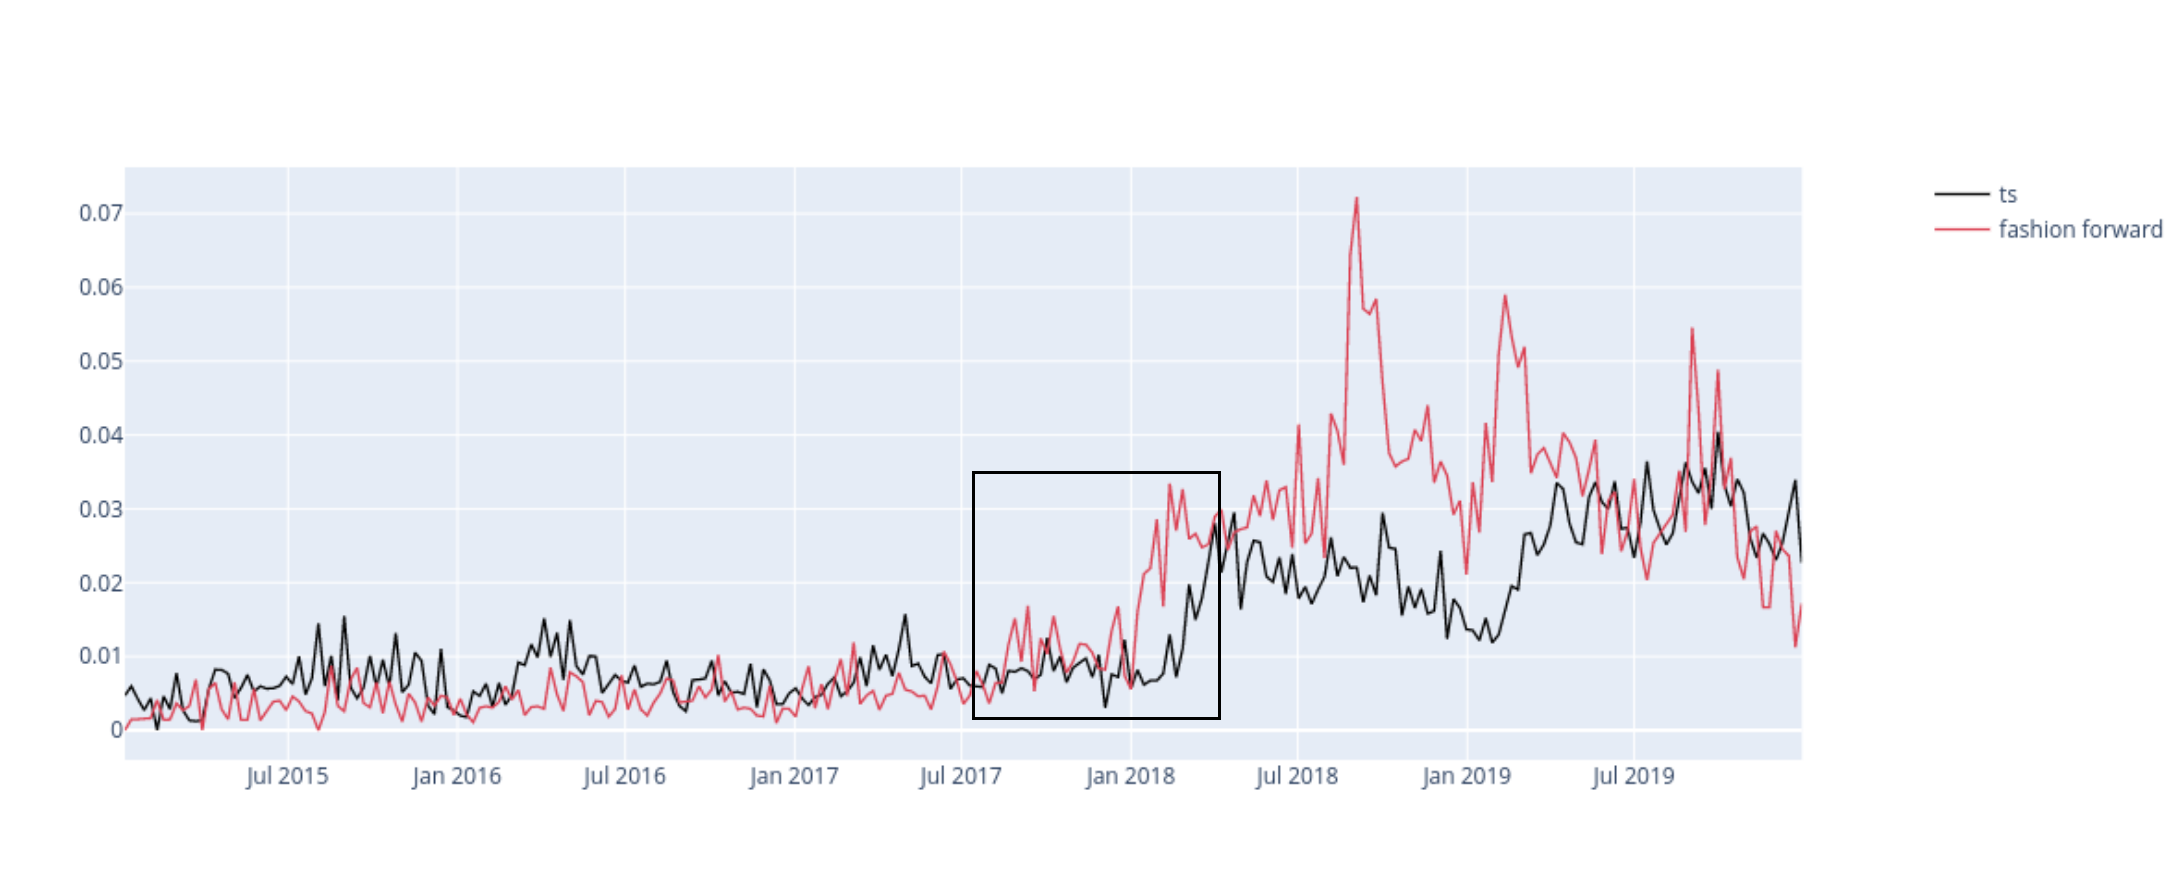
\includegraphics[width=1.\linewidth]{figure/emerging_trend}
  \caption{A shoes trend of our dataset. In black the main signal and in red its associated \textit{fashion-forward} weak signal. The Gap between our two signals in the end of 2017/beginning of 2018 announces the future explosion of the fashion trend.}
\label{fig:oneemergingtrend}
\end{figure}





\section{Experimental results}
\label{sec:exp}
%In this section, we evaluate how our hybrid framework is able to deal with the fashion dataset and leverage our complex external weak signals. To lead our experience, we keep hide the last year of each time series as our test set. For each method and each time series, based on the first five years of data, we predict the last year and compute our accuracy on it.

\subsection{Training}

To train our hybrid model, we split our dataset into three blocks, train, eval and test sets. We use the 3 first years as our train set, we keep the 4th year for our eval set and we hide the last year for our test set. We train our hyrid model to compute a one-year ahead prediction, $\lag$ equal to 52, and we set the window size $\window$ equal to 104.
Using the two first year of our train set, we fit a first per-time-series parametric model for each time series. With the resulting collection of local models, we compute a first forecast of the third year for each sequence. Using these forecasts, we preprocess our time series and finally determine our RNN inputs. We can, then, train our RNN at understanding and correcting the previous collection of parametric model's forecasts. In the same way, for the eval set, we fit a second time our per-time-series predictors using the three first years and we forecast the fourth year. We preprocess our time series and we evaluate how our error-corrector RNN is able to improve the first collection of predictions of the fourth year.
At the end, we repeat the same process for the fifth year and compute our final accuracy measures. An example of our temporal split is shown in  Figure~\ref{fig:train_eval_test_set}.
%We train our hyrid model to compute a one-year ahead prediction with $\window$ equal to 104 and a $\lag$ equal to 52. For each time series, we fitted 3 per-time-series parametric models: We fit the first one using the 2 first years and compute a forecast of the thrid year. 

%In order to increase our train set, we use a moving window that provide 53 input/output couples per sequences, being 530000 couples in total. 

For the first parametric per-time-series models, we used existing Python or R librarys to estimate the different parameters $\statparam^n$. During the M4 competition, parameters of the exponential smoothing of the porposed hybrid model could move during the training. In our framework,
$\{\statparam^n\}_{1\leqslant n \leqslant N}$ are fixed during the training of the recurrent models. In this section we propose two versions of HERMES depending of the choice of local parametric models. The first one use as predictors an additive exponential smoothing model as a reference close to \cite{smyl2020hybrid}. The second one use as predictors the TBATS model of \cite{doi:10.1198/jasa.2011.tm09771} and  achieves striking accuracy results on our fashion dataset. For the neural network part, we built an architecture summarized in Figure~\ref{fig:rnn_architecture}. It is composed of 3 LSTM layer of shape 50 and a final Dense layer to provide the correct output dimension. We use a classical Adam optimizer with a learning rate equal to 0.005 and a batch size equal to 64. For our loss function, we tested several metrics and we finally converged on the following one :

$$
l(\ts^n_{T+1:T+\lag},\tspred^n_{T+1:T+\lag|T}) = \frac{\sum_{i=1}^{\lag}|\ts^n_{T+i} - \tspred^n_{T+i|T}|}{\meants^n_T}
$$
%


All our code is developed in Python using the Tensorflow library. It allows the use of a GPU to speed up the trainig process.



\begin{figure}
  \centering
    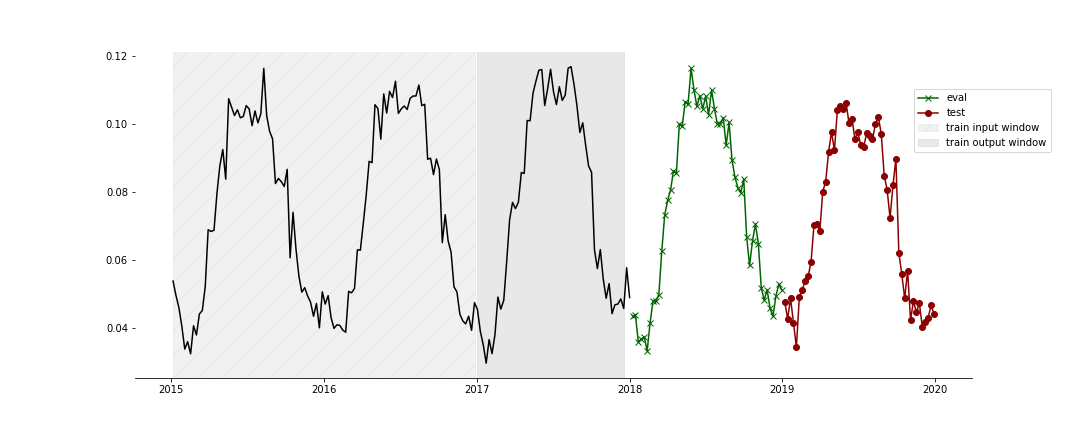
\includegraphics[width=1.\linewidth]{figure/train_eval_test_set}
  \caption{Temporal split for our training process}
\label{fig:train_eval_test_set}
\end{figure}

\begin{figure}
  \centering
    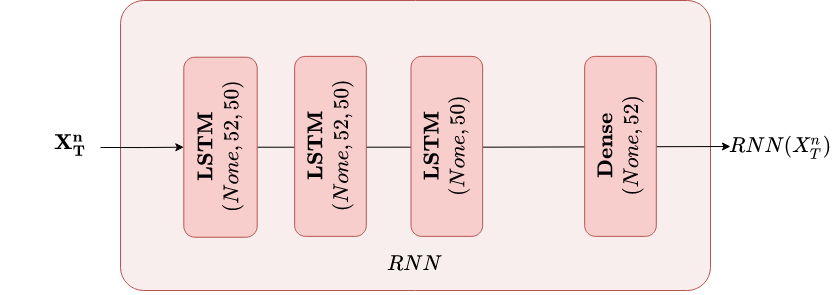
\includegraphics[width=0.8\linewidth]{figure/lstm_archi}
  \caption{$\classifier$ and $\predictor$ architecture.}
\label{fig:rnn_architecture}
\end{figure}


%To train our hybrid models, we made the choice of don't using the original code of the hybrid method provided during the M4 competition. Indeed, the proposed implementation is difficult to use in a more general framework and it is quite slow because it doesn't enable the use of GPU. Thereby, we propose with this paper, a new version of the hybrid framework, including the original multiplicative model and the new additive one. 
%Our code is developed in Python using the Tensorflow library and it allows the use of a GPU to speed up the training process contrary to other methods \textcolor{red}{\cite{} developed for the M4 competition}. In addition, our approach offers the possibility of providing forecasts for a totally  new collection of sequences without retraining the entire hybrid model. Given a new time series,  the weights of the error-corrector recurrent model are frozen and only the new time-series-specific statistical model has to be trained.% It remains the responsibility of the users to provide new sequences sharing same behaviours than the dataset using for the training to keep the same accuracy level.

%For more details about the general hybrid training, a complete description of the training process can be found in the M4 hybrid model paper or in an interesting application of the method on electric load forecasting, see \citep{dudek2020hybrid}.

%\textcolor{red}{Detail here or in the appendix the training details: number of samples, optimizers, learning rates, etc.}

%\vspace{.2cm}

%\textcolor{red}{Detail Train/test split.}

\subsection{Benchmarks, hybrid models and Metrics}

As benchmarks, we chose several well-known statistical methods and deep learning approaches. Using the R package \texttt{forecast} and the Python packages \texttt{statsmodels},  \texttt{tbats} , we compute for each time series a prediction with the following methods: \textit{snaive}, \textit{ets}, \textit{stlm}, \textit{thetam}, \textit{tbats} and \textit{auto.arima}. The forecast of the \textit{snaive} method is only the repetition of the last same past period. \textit{ets} model is an additive exponential smoothing with a level component and a seasonal component. \textit{stlm} approach uses a multiplicative decomposition and models the seasonally adjusted time series with an exponential smoothing model. \textit{Thetam} model decomposes the original signal in $\theta$-lines, predicts each one separately and recomposes them to produce the final forecast. \textit{tbats} is a powerful statistical model using a trigonometrical seasonality modelization. The last one \textit{auto.arima} is the R implementation of the ARIMA model with an automatic selection of the best parameters. A complete description and references for these models can be found in \citep{hyndman2020package}. As a deep learning approach, we considered a full LSTM (\textit{lstm}) neural network composed of 3 LSTM layers of shape 50 and a final Dense layer of shape 52.

Against these models, we propose two versions of HERMES called respectively \textit{hermes-ets} and \textit{hermes-tbats} according to the per-time-series model choice.
%Against these models, we propose two versions of our regime switching hybrid recurrent model \textit{rshm}. The first one, that we name \textit{rshm-ets}, is the hybrid model with an additive exponential smoothing model as parametric model. For the second one, we use the TBATS approach as paramteric model and we named it \textit{rshm-tbats}. 
%To reach a higher accuracy level we also propose an ensembling (\textit{ensembling} of our hybrid approach using the FFORMA method created during the M4 competition, see \citep{fforma}).  
Moreover, we evaluate our hybrid framework with the inclusion of our weak signals (ws) referred to as \textit{hermes-ets-ws} and \textit{hermes-tbats-ws}. In order to provide a fair comparison, we also train a \textit{lstm} with the weak signals named \textit{lstm-ws}.

To compare the different methods, we use the same metrics as in the M4 competition: the Mean Absolute Scaled Error (MASE), the Symmetric Mean Absolute Percentage Error (sMAPE) and the final M4 competition metric, the Overall Weighted Average (OWA) of the sMAPE and the MASE defined as follows:
\begin{align*}
\mathrm{MASE} &= \frac{T-m}{h}\frac{\sum_{i=1}^h |Y_i - \hat{Y}_i| }{\sum_{i=1}^{T-m} |Y_i - Y_{i-m}|}\,,\\
\mathrm{sMAPE} &= \frac{1}{h} \sum_{i=1}^h \frac{2|Y_i - \hat{Y}_i|}{|Y_i| + |\hat{Y}_i|}\,,\\
\mathrm{OWA} &= \frac{1}{2}\left(MASE/MASE_{snaive} + sMAPE/sMAPE_{snaive}\right)\,,
\end{align*}

where $\hat{Y}$ is a model prediction, $\lag$ is the horizon, $m$ the seasonality and $MASE_{snaive}$ is the $MASE$ computed with the $snaive$ model prediction, idem for the $sMAPE_{snaive}$.

Detecting emerging and declining trends is a crucial issue for the fashion industry. A correct or incorrect prediction could lead to good returns or massive waste due to overstock or unsold clothes. In a given year, we define an increasing trend as a trend that does more than 10\% of growth in terms of Year and Year. In the same way, we define a decreasing trend as a trend that declines by 10\% or more. We classify other trends as flat trends. On the test set, the year 2019, we have 1871 increasing trends, 2016 decreasing trends and 6113 flat trends. In addition to the accuracy metrics, we also compare the different methods on this classification task and especially difference between methode using weak signal or not.



%As detecting emerging and declining trends is a fondamental issue that is facing the fashion industry, we evaluate also the different methods on this task. In a given year, we define an increasing trend as a trend that do more than 10\% of growth in term of Year and Year.A decreasing trend is a trend that decline of -10\% or more. We classify the other trend as flat trend. On the test set, the year 2019, we have 1871 increasing trends, 2016 decreasing trends and 6113 flat trends. We evaluate all the methods on this classification task.



%\textcolor{red}{where $\mathrm{smape_{snaive}}$ and $\mathrm{mase_{snaive}}$ are}.

%\subsection{Results for XXX Dataset}
%\textcolor{red}{If possible, a few results of the hybrid approach without weak signals on a dataset other than Heuritech.}






\subsection{Result for Heuritech Fashion dataset}

%\textcolor{red}{Add a figure of a time series with all models (and others in Appendix).}

%\vspace{.2cm}

%\textcolor{red}{Add a table with the results on the trends classifications used in Heuritech.}

%\textcolor{blue}{Result on 1000ts}  \\

\textbf{10000 Heuritech Fashion time series global accuracy}

For our 3 metrics and for each model, we compute the average on all our sequences \numberts~  on the final year. Results are displayed in the Table~\ref{tab:metricresults}. For our model using neural networks, we trained 10 models with different seeds and compute the average and the standard deviation for the three metrics. For the statistical models, we can see a large domination of the TBATS model with an OWA equal to 0.850. It is one of the main motivations why we use this model on our best HERMES candidate as the predictor model. However, we can see that the full LSTM model \textit{lstm} is the best model over our benchmark candidates with a OWA equal to 0.825.

Considering our new HERMES approach, we see a large domination of our \textit{hermes-tbats} version with a OWA equal to 0.816 and a strong stability across the different trainings. Regarding \textit{hermes-ets}, we see a huge increase compared to its predictor choice \textit{ets} with a descrease from 0.937 to 0.875 in term of OWA. However, its accuracy remains low in comparison to the \textit{lstm} benchmarck or our HERMES's second version using Tbats. In Figure~\ref{fig:hybrid-examples}, we displayed some examples of \textit{hermes-tbats} model and some weaknessess that it is able to understand and accurately correct.

\begin{table*}
  \caption{Results summary on our 10000ts Fashion dataset. For each metric, we compute the average on all our time series. For our approaches using neural network, we trained 10 models with different seeds and we display the mean and the standard deviation of our 10 results.}
  \centering
  \resizebox{1.2\width}{!}{
  \begin{tabular}{l||llllllllll}
   &&\multicolumn{2}{c}{\textbf{MASE}} && \multicolumn{2}{c}{\textbf{SMAPE}} && \multicolumn{2}{c}{\textbf{M4}}& \\
    &&  \textit{mean}  & \textit{std} && \textit{mean}  & \textit{std} && \textit{mean}  & \textit{std} \\
    \hline
	\hline
	\rule{0pt}{2ex} \\
     \textit{snaive} && 0.881 & - && 25.27 & - && 1. & -\\
     \textit{thetam}  && 0.844 & - && 24.17 & - && 0.970 & -\\
     \textit{arima} && 0.826 & - && 23.63 & - && 0.949 & -\\
     \textit{ets} && 0.807 & - && 23.58 & - && 0.937 & -\\
     \textit{hermes-ets-ws} && 0.769 & 0.004 && 22.69 & 0.126 && 0.901 & 0.007\\
     \textit{stlm} && 0.770 & - && 22.05 & - && 0.882 & -\\
     \textit{hermes-ets} && 0.759 & 0.001 && 22.16 & 0.026 && 0.875 & 0.001\\
     \textit{tbats} && 0.745 & - && 21.13 & - && 0.850 & -\\
     \textit{lstm-ws} && 0.728 & 0.004 && 20.18 & 0.085 && 0.837 & 0.004\\
     \textit{lstm} && 0.724 & 0.003 && 20.08 & 0.052  && 0.825 & 0.004\\
     \textit{hermes-tbats-ws} && 0.713 & 0.005 && 20.53 & 0.170 && 0.825 & 0.009\\
     \textbf{\textit{hermes-tbats}} && \textbf{0.715} & 0.002 && \textbf{20.41} & 0.056 && \textbf{0.816} & 0.002\\
    %\hline
  \end{tabular}
  }
\label{tab:metricresults}
\end{table*}

\begin{figure}
  \centering
    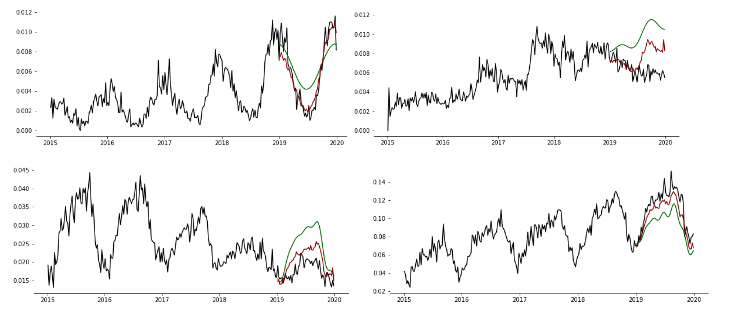
\includegraphics[width=1.\linewidth]{figure/hybrid_model_examples}
  \caption{\textit{hermes-tbats} forecast examples. In green the prediction of the per-time-series predictors \textit{tbats}. In red the final forecast of our hermes hybrid model \textit{hermes-tbats}.}
\label{fig:hybrid-examples}
\end{figure}


\textbf{10000 Heuritech Fashion time series classification task}

An interesting constat is that models using our weak signals slightly underperform their relative without-weak-signals models on all our 3 metrics. We see an exception for our \textit{hermes-tabts-ws} that outperform its relative \textit{hermes-tabts} in term of MASE (0.713 compare to 0.715) but it is not clearly significative compare to the standard deviation. The impact of our weak signal is revealed with our classification results.

When we compare our classification results between the \textit{tbats} model and our hybrid method \textit{hermes-tbats} given in Table~\ref{tab:tbatsclass}, we note an impresive diminution of that we called an "unforgiveable error" : forecast an increase instead of a decrease and vice versa. We divide the number of this error by 3 with only a slightly decrease of the number of correct increase/decrease predictions. However, with our weak signals, we see that \textit{hermes-tbats-ws} is able to catch twice as much as its relative model without weak signal while keeping a relatively low number of "unforgivable error".

When we look at the result of \textit{lstm-ws} and \textit{lstm} displayed in Table~\ref{tab:lstmclass}, we can also note an rise of the number of correct prediction but with an important increase of the number of classification errors.


\begin{table}
  \caption{\textit{tbats}, \textit{hermes-tbats} and \textit{hermes-tbats-ws} models confusion matrix}
  \vspace{0.2cm}
  \centering
  \vspace{0.2cm}
  \par \textit{tbats} model confusion matrix\\
  \vspace{0.2cm}
  \resizebox{1.2\width}{!}{
  \begin{tabular}{l||llll}
    && pred-dec  & pred-flat & pred-inc  \\
    \hline
    \hline
    \rule{0pt}{2ex} \\
	true-dec && 327 & 1607 & 82 \\
    true-flat && 195 & 5586 & 232 \\
    true-inc && 68 & 1585 & 318 \\
  \end{tabular}
  }
  \vspace{0.2cm}
  \par \textit{hermes-tbats} model confusion matrix\\
  \vspace{0.2cm}
  \centering
  \resizebox{1.2\width}{!}{
  \begin{tabular}{l||llll}
    && pred-dec  & pred-flat & pred-inc  \\
    \hline
    \hline
    \rule{0pt}{2ex} \\
	true-dec && 250 & 1747 & 19 \\
    true-flat && 131 & 5802 & 80 \\
    true-inc && 33 & 1639 & 299 \\\
  \end{tabular}
  }
  \centering
  \vspace{0.2cm}
  \par \textit{hermes-tbats-ws} model confusion matrix\\
  \vspace{0.2cm}
  \resizebox{1.2\width}{!}{
  \begin{tabular}{l||llll}
    && pred-dec  & pred-flat & pred-inc  \\
    \hline
    \hline
    \rule{0pt}{2ex} \\
	true-dec && 615 & 1365 & 36 \\
    true-flat && 510 & 5374 & 129 \\
    true-inc && 65 & 1444 & 462 \\
  \end{tabular}
  }
\label{tab:tbatsclass}
\end{table}



\begin{table*}
  \caption{\textit{lstm} and \textit{lstm-ws} model confusion matrix}
  \vspace{0.2cm}
  \centering
  \vspace{0.2cm}
  \par \textit{lstm} model confusion matrix\\
  \vspace{0.2cm}
  \resizebox{1.2\width}{!}{
  \begin{tabular}{l||llll}
    && pred-dec  & pred-flat & pred-inc  \\
    \hline
    \hline
    \rule{0pt}{2ex} \\
	true-dec && 447 & 1539 & 30 \\
    true-flat && 444 & 5324 & 245 \\
    true-inc && 66 & 1410 & 495 \\
  \end{tabular}
  }
  \centering
  \vspace{0.2cm}
  \par \textit{lstm-ws} model confusion matrix\\
  \vspace{0.2cm}
  \resizebox{1.2\width}{!}{
  \begin{tabular}{l||llll}
   	&& pred-dec  & pred-flat & pred-inc  \\
    \hline
    \hline
    \rule{0pt}{2ex} \\
	true-dec && 796 & 1161 & 59 \\
    true-flat && 1053 & 4701 & 259 \\
    true-inc && 90 & 1259 & 622 \\
  \end{tabular}
  }
\label{tab:lstmclass}
\end{table*}
%Table~\ref{tab:metricresults} summarize the results of all our benchmark models and our 2 hybrid methods for the 3 metrics described above. Values are errors averaged over our \numberts on the test set. For the statistical models, we can see a large domination of the TBATS model with an OWA equal to 0.847. It is one of the main reasons why we use this model on one of our hybrid frameworks as the parametric model. However, we can see that the full LSTM model \textit{lstm} is the best model over our benchmark candidates. This result shows that, with a large dataset, deep learning models can outperform the traditional approaches on average. An example of prediction of all the benchmark methods is displayed in the Figure~\ref{fig:forecastexample}.Our two different regime switching hybrid models achieve a higher level of accuracy compared to their references. For the \textit{rshm-ets}, we pass from ??? for the \textit{ets} model alone to ???? for the hybrid model. Its $\classifier$ threshold $\threshold$ was fixed at ???. With this threshold, the error-corrector model correct ???? sequences of the $\numberts$. On these corrected time series, compared to the \textit{ets} approach, our approach MASE falls from ??? to ???. However \textit{rshm-ets} doesn't succeed at outperforming some of the benchmark models, for example \textit{tbats} of \textit{lstm}. The \textit{rshm-tbats} version clearly outperforms all the previous models. Based on a \textit{tbats} model, which already achieves an interesting level of accuracy, \textit{rshm-tbats} reach the higher level with a MASE equal to 0.728 and and the lower OWA equal to 0.840. With a threshold fixed at 0.5, this version of our hybrid framework corrects 294 TBATS predictions. On these 294 trends, the \textit{tbats} has an OWA equal to 0.867 and with the regime switching model correction, we reach an OWA equal to 0.845. An example of prediction of our two regime-switching hybrid recurrent model is presented in the Figure~\ref{fig:hybridforecast}. Other additional examples and results can be found in Appendix.

%\begin{figure}
%  \centering
%    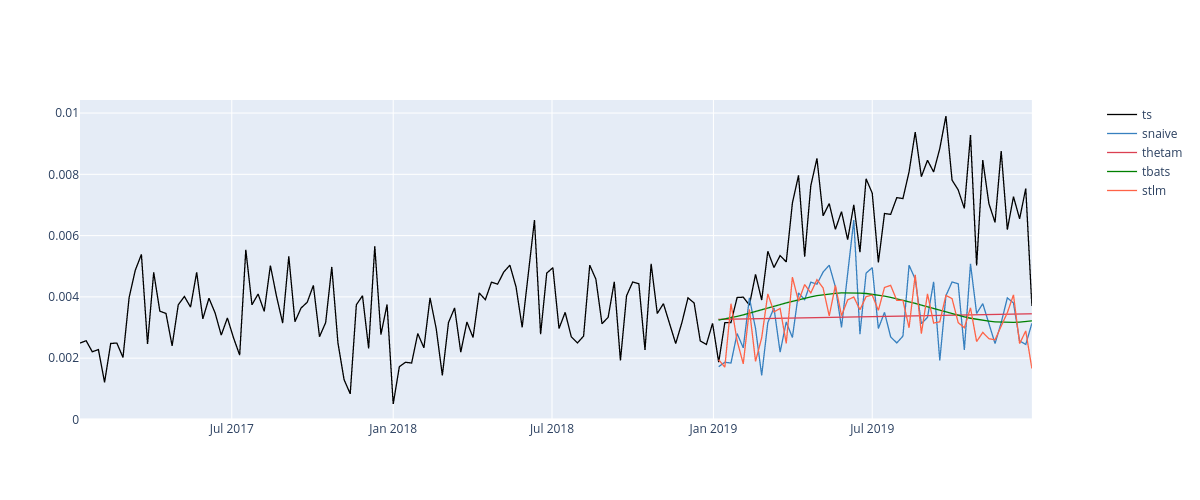
\includegraphics[width=1.\linewidth]{figure/example_prediction}
%  \caption{Example of benchmarck models's predictions on an emerging trend}
%\label{fig:forecastexample}
%\end{figure}

%\begin{figure}
%  \centering
%    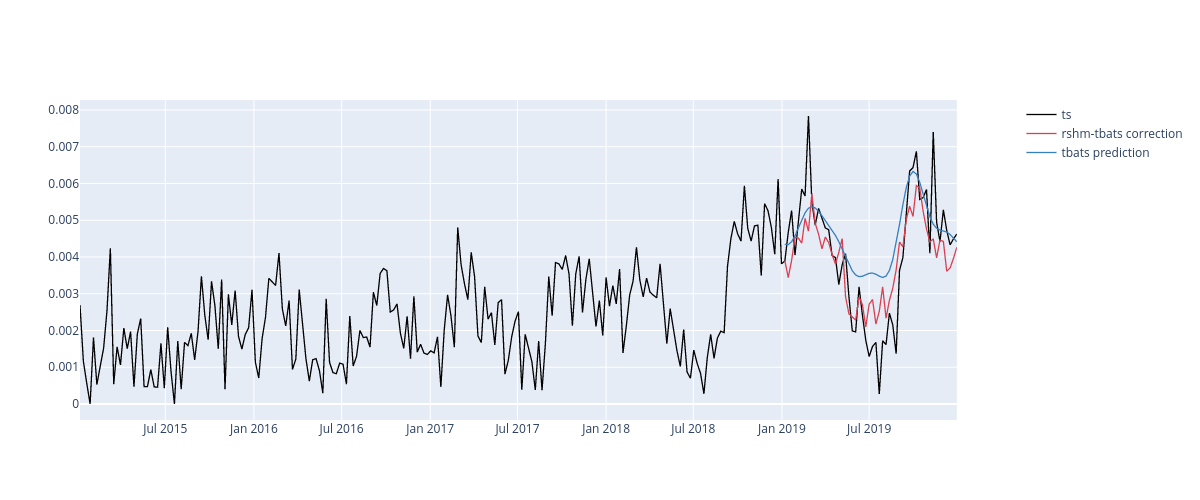
\includegraphics[width=1.\linewidth]{figure/rshm_tbats_prediction_example}
%  \caption{Example of the \textit{rshm-ets} model prediction. In blue the ets reference and in red the $\predictor$ correction. $%\classifier$ return ??? that is greater than its threshold ???: we use then the correction.}
%  \centering
%    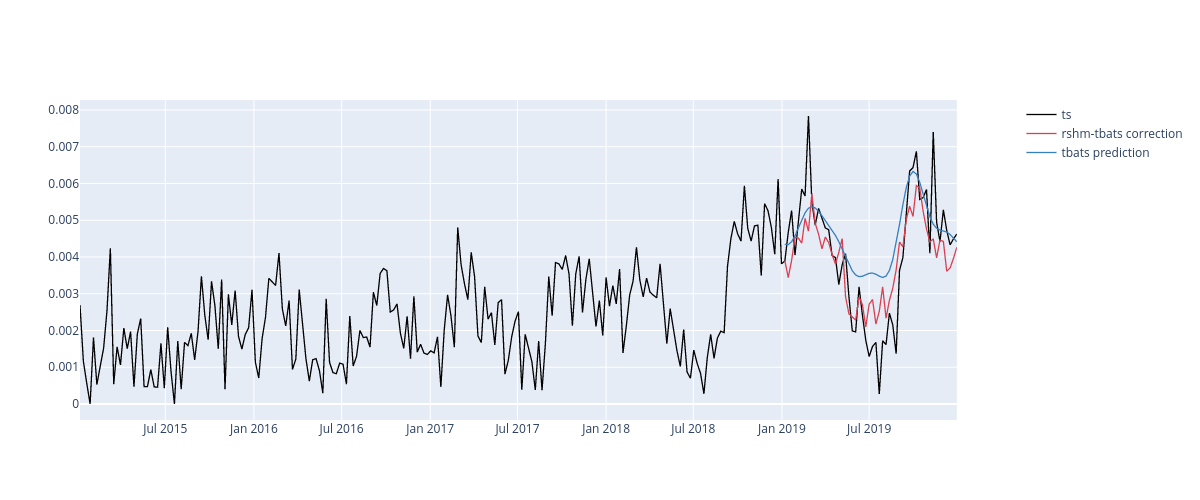
\includegraphics[width=1.\linewidth]{figure/rshm_tbats_prediction_example}
%  \caption{Example of the \textit{rshm-tbats} model prediction. In blue the Tbats reference and in red the $\predictor$ correction. $\classifier$ return 0.537 that is greater than its threshold 0.5: we use the RNN correction.}
%\label{fig:hybridforecast}
%\end{figure}

\textbf{Importance of the size of the dataset}

In addition to our results on our fashion dataset gathering 10000 time series, we also investigate the behaviours of our HERMES model when it is trained on smaller datasets. We did 2 experiences, we train our models on a dataset of 1000 time series and on a dataset of 100 time series. Results are given in Table~\ref{tab:1000metricresults} and Table~\ref{tab:100metricresults}.

With these investigations, we can make two important remarks. First, our hybrid framework \textit{hermes-tbats} achieves the first position in term of global accuracy on both datasets. Due to the strengh of its per-time-series predictor TBATS, our hybrid model succeds at correcting some of its weaknesses and logically reach a striking final accuracy. Secondly, we can note that the accuracy of the full neural network \textit{lstm} decrease according to the dataset size. With a small dataset of 100 time series, a local statistical model like \textit{tbats} or \textit{stlm} can largely outperform its accuracy level. In fact, learn how to compute a full prediction from scratch is a complex task and for a neural network, it evolves a large amout of data. Nevertheless, with our hybrid framework, the RNN task is largely simplify. Our achitectures logicaly needs less data to be train and perform well.


\begin{table*}
  \caption{Results summary on our 1000ts Fashion dataset.For each metric, we compute the average on all our time series. For our two apporaches using neural network, we trained 10 models with different seeds and we display the mean and the standard deviation of our 10 results.}
  \centering
  \resizebox{1.2\width}{!}{
  \begin{tabular}{l||llllllllll}
   &&\multicolumn{2}{c}{\textbf{MASE}} && \multicolumn{2}{c}{\textbf{SMAPE}} && \multicolumn{2}{c}{\textbf{M4}}& \\
    &&  \textit{mean}  & \textit{std} && \textit{mean}  & \textit{std} && \textit{mean}  & \textit{std} \\
    \hline
	\hline
	\rule{0pt}{2ex} \\
     \textit{snaive} && 0.871 & - && 25.29 & - && 1. & -\\
     \textit{thetam}  && 0.849 & - && 24.58 & - && 0.980 & -\\
     \textit{arima} && 0.821 & - && 23.69 & - && 0.951 & -\\
     \textit{ets} && 0.801 & - && 24.18 & - && 0.944 & -\\
     \textit{stlm} && 0.765 & - && 22.22 & - && 0.885 & -\\
     \textit{lstm-nows} && 0.740 & 0.007 && 20.56 & 0.154 && 0.856 & 0.008\\
     \textit{tbats} && 0.734 & - && 21.19 & - && 0.847 & -\\
     \textbf{\textit{hybrid-nows}} && \textbf{0.719} & 0.002 && \textbf{20.79} & 0.094 && \textbf{0.833} & 0.004\\
  \end{tabular}
  }
\label{tab:1000metricresults}
\end{table*}

%\begin{table*}
%  \caption{Results summary on our 1000ts Fashion dataset.For each metric, we compute the average on all our time series. For our two apporaches using neural network, we trained 10 models with different seeds and we display the mean and the standard deviation of our 10 results.}
%  \centering
%  \begin{tabular}{lllllll}
%    \hline
%    &  MASE-mean  & MASE-std & SMAPE-mean & SMAPE-std & OWA-mean & OWA-std  \\
%    \hline
%     \textit{snaive} & 0.871 & - & 25.29 & - & 1. & -\\
%     \textit{thetam}  & 0.849 & - & 24.58 & - & 0.980 & -\\
%     \textit{arima} & 0.821 & - & 23.69 & - & 0.951 & -\\
%     \textit{ets} & 0.801 & - & 24.18 & - & 0.944 & -\\
%     \textit{hybrid-nows-ets} & 0.768 & 0.002 & 22.91 & 0.111 & 0.902 & 0.005\\
%     \textit{stlm} & 0.765 & - & 22.22 & - & 0.885 & -\\
%     \textit{lstm-nows} & 0.740 & 0.007 & 20.56 & 0.154 & 0.856 & 0.008\\
%     \textit{tbats} & 0.734 & - & 21.19 & - & 0.847 & -\\
%     \textit{hybrid-nows} & 0.719 & 0.002 & 20.79 & 0.094 & 0.833 & 0.004\\
%    \hline
%  \end{tabular}
%\label{tab:metricresults}
%\end{table*}
\begin{table*}
  \caption{Results summary on our 100ts Fashion dataset. For each metric, we compute the average on all our time series. For our two apporaches using neural network, we trained 10 models with different seeds and we display the mean and the standard deviation of our 10 results.}
  \centering
  \resizebox{1.2\width}{!}{
  \begin{tabular}{l||llllllllll}
   &&\multicolumn{2}{c}{\textbf{MASE}} && \multicolumn{2}{c}{\textbf{SMAPE}} && \multicolumn{2}{c}{\textbf{M4}}& \\
    &&  \textit{mean}  & \textit{std} && \textit{mean}  & \textit{std} && \textit{mean}  & \textit{std} \\
    \hline
	\hline
	\rule{0pt}{2ex} \\
     \textit{snaive} && 0.876 & - && 26.98 & - && 1. & -\\
     \textit{thetam}  && 0.823 & - && 25.11 & - && 0.944 & -\\
     \textit{arima} && 0.814 & - && 24.61 & - && 0.940 & -\\
     \textit{lstm-nows} && 0.767 & 0.045 && 22.22 & 0.848 && 0.877 & 0.051\\
     \textit{stlm} && 0.742 & - && 23.03 & - & 0.863 & -\\
     \textit{tbats} && 0.745 & - && 22.16 & - & 0.856 & -\\
     \textbf{\textit{hybrid-nows}} && \textbf{0.739} & 0.003 && \textbf{22.31} & 0.083 && \textbf{0.845} & 0.003\\
  \end{tabular}
  }
\label{tab:100metricresults}
\end{table*}


%The Table~\ref{tab:metricresultsws},Table~\ref{tab:etsclass} and Table~\ref{tab:tbatsclass} presents how our candidates are able to understand and leverage our weak signals in terms of accuracy and classification. The full lstm approach shows a slight increase, from 0.872 to 0.867 for the OWA metric, and correctly predicts 4 increasing/decreasing trends. \textcolor{blue}{No for now, WIP} A real improvement is shown by our proposed regime switching framework. With a threshold fixed at 0.465, this version of our hybrid framework corrects 118 TBATS predictions. On these 118 trends,   the \textit{tbats} has an OWA equal to 0.893 and with the regime switching model correction, we reach an OWA equal to 0.868.




%In a first place, Table 2 shows the final accuracy of the statistical models, the LSTM model and our 2 hybrid models without external data. Even without the weak signals, our 2 hybrid approaches largely outperform the statistical references. The multiplicative model show the best accuracy with a OWA equal to 0.875. We can note that the additive model slightly under-performs the traditional multiplicative one on average. This doesn't show a weakness of the additive version but more that a large part of our dataset is more-suited for multiplicative modelization. At the end, the strength of training both methods, additive and multiplicative, is in the final porposed ensembling \textit{ensembling} that combines the two approaches with the FForma ensembling.

%In a second place, Table 3 shows the evaluation of our 4 trained hybrid models: the 2 previous ones without weak signals, and our 2 full hybrid models with weak signals. We present also the accuracy of a simple LSTM model with and without weak signals. We can show the impressive improvement due to our external signals. Again, the multiplicative method achieves the best accuracy with OWA metric equal to 0.860. We propose like previously, an ensembling mixing our two full hybrid models with weak signals and it reach the high level of accuracy with an OWA equal to 0.849.

%In a third place, table 4 presents the result of our inference process. We split our dataset in five equal parts of 2800 sequences and hide the last year for each trends. Then, like a cross validation, we train a model on 4 parts and compute its accuracy on the last one on the last year. The model never saw the last part so we use our inference process to compute predictions. With a permutation of the parts, we can repeat the process and train 5 models, each trained on a specific pool of 4 parts and tested on the remaining part of the dataset. For each hybrid model (additive/multiplicative with and without weak signals) Table 4 shows the average accuracy and the Standard Deviation of the 5 trained hybrid models. We can see that our inference process achieve really accurate results and practically the same that our hybrid models trained on the entire dataset. These results prove that, even without having seen a sequence during the training, if the time series share same behaviours that the training sample, our hybrid approaches can perfectly compute accurate predictions. Furthermore, the Standard Deviation is really low for all our metrics. This result shows that our hybrid framework is robust and reach constant accuracy level on large dataset.


\subsection{Discussion}
\label{sec:discussion}

%With our results, we can make two interesting conclusions. Firstly, the regime switching hybrid framework is a really promising framework. By mixing the performance of local parametric models and a global DNN, our two versions clearly outperform traditional statistical methods. Furthermore, this framework is totally suited for dealing with external signals. With a fine pre-processing and a well-designed architecture, our two models succeed at leveraging our complex extra data and reach impressive accuracy levels. Secondly, our results bring to light the quality of our new Fashion dataset. We saw that the full LSTM model \textit{lstm} outperforms all time series specific models. This shows that our dataset is well suited to train complex neural network architectures able to learn information cross sequences. With the addition of our weak signals, we give a totally new dimension to our fashion dataset. Our results show that our external weak signals hide a complex but usable predictive power by DNN architecture. By making it publicly available, we hope that it will enhance the set of datasets for time series forecasting.

With our results, we can make several interesting conclusions. Firstly, our new HERMES framework is a really promising framework. By mixing the performance of local parametric models and a global DNN, our \textit{hermes-tbats} version clearly outperform traditional statistical methods and full neural network models. Furthermore, this framework is totally suited for dealing with external signals. With a fine pre-processing and a well-designed architecture, our hybrid framework succeed at leveraging our complex extra data and reach impressive accuracy level in term of classification. Secondly, our results bring to light the quality of our new Fashion dataset. We saw that the full LSTM model \textit{lstm} outperforms all time series specific models when it is trained with the biggest dataset of 10000 time series but not with the smaller ones. This shows that complex neural network architectures involve large amount of data to be train and our full dataset is well suited for this. Finally, with the addition of our weak signals, we give a totally new dimension to our new hybrid architecture and our fashion dataset. Our results show that our external weak signals hide a complex but usable predictive power by our HERMES model. However, we believe that it remains a lot of ways to explore in order to leverage the full potential of these chaotic signals.

%\begin{table*}
 % \caption{Comparison between our hybrid models without and with our external weak signals, (Mean/Median)}
  %\label{sample-table}
  %\centering
  %\begin{tabular}{lllllll}
   % \hline
    %&  MASE  & MASE-std & SMAPE & SMAPE-std & OWA & OWA-std \\
    %\hline
    %lstm & 0.881/0.824 & 0.34 & 24.41/21.56 & 12.81 & 0.895/0.885 & 0.11 \\
    %lstm-ws & 0.869/0.814 & 0.33 & 24.56/21.33 & 14.40 & 0.890/0.874 & 0.132 \\
    % hybrid-add & 0.863/0.812  & 0.32 & 24.17/21.36 & 13.0 & 0.877/0.880 & 0.08 \\
     %hybrid-mul & 0.858/0.817 & 0.30 & 24.06/21.30 & 13.0 & 0.876/0.873 & 0.11 \\
  %   hybrid-add-ws & 0.852/0.807 & 0.30 & 24.03/21.17 & 13.0 & 0.872/0.869 & 0.10 \\
%     hybrid-mul-ws & 0.836/0.798 & 0.29 & 23.67/20.87 & 12.9 & 0.860/0.858 & 0.12 \\
 %    Ensembling & 0.827/0.787 & 0.29 & 23.43/20.63 & 12.8 & 0.849/0.849 & 0.11\\
  %  \hline
  %\end{tabular}
%\end{table*}



%\begin{table*}
 % \caption{Cross-Validation. we split our dataset in 5 equal parts. We train for each hybrid approach, 5 models on 4 specific parts of the dataset and we test them of the remaining parts with our inference process.}
  %\label{sample-table}
  %\centering
 % \begin{tabular}{lllllll}
  %  \hline
   % &  MASE  & MASE-std & SMAPE & SMAPE-std & OWA & OWA-std \\
   % \hline
   %  hybrid-add & 0.861  & 0.004 & 24.16 & 0.18 & 0.877 & 0.002 \\
   %  hybrid-mul & 0.856 & 0.008 & 23.95 & 0.25 & 0.870 & 0.005 \\
   %  hybrid-add-ws & 0.848 & 0.004 & 24.00 & 0.18 & 0.869 & 0.002 \\
   %  hybrid-mul-ws & 0.844 & 0.010 & 23.74 & .20 & 0.863 & 0.006 \\
   % \hline
  %\end{tabular}
%\end{table*}




\section{Conclusion}
\label{sec:conclusion}
%In this paper, we propose the first hybrid model including external weak signals for time series forecasting. We show that hybrid framework is a really promising way. With its extended error-corrector DNN part, it is clearly well-suited for dealing with any kind of external signals in order to correct weaknesses of first parametric models. Furthermore, With our additive version, we show that the hybrid model is not frozen in it original form. Thereby, future research explorations would be to improve its framework with new per-time-series approaches and test new error-corrector DNN part like the recent Transformer model.

In this paper, we propose the first hybrid model including external weak signals for time series forecasting. We show that hybrid framework is a really promising way and with its extended error-corrector DNN part, it is clearly well-suited for dealing with any kind of external signals. Furthermore, our general framework shows that the hybrid model is able to include any kind of any per-time-series models. Depending of the use cases, the nature of the observed time series, users can choose the best parametric models, correct some of its weaknessess and finally increase its accuracy with the HERMES framework. Thereby, future research explorations would be to evaluate its framework with a large collection of per-time-series approaches and understand relationships between first parametric model choice and final hybrid model accuracy. Is it the best parametric model always the best choice in our HERMES framework ? A other promising exploration would be to challenge the error-corrector DNN model with an other one using Transformer or a collection of DNN specialized on specific kind of weaknessess.

With this first contribution, we join the first fashion dataset gathering \numberts\ fashion times series and a complex collection of external signals. We believe that this dataset hide really fine dynamics and interactions where complex models would express their potential. By making it publicly available, we hope that it will enhance the set of datasets for time series forecasting and pave the way for further explorations.


\bibliography{hermes_paper}
\bibliographystyle{apalike}

\appendix

%\section{Fashion Dataset overview}



%\section{Hidden regime algorithm}
%
%In our framework, we assume that our sequence are generated with 2 hidden regime. As this regime, noted $\hiddenregime$, is never observed, we use the Expectation Maximization (EM) algorithm to write our loss function:
%%We note $\rnnparam^{(t)} = \{\rnnparam_c^{(t)},\rnnparam_p^{(t)}\}$ the weights of $\classifier$ and of $\predictor$ at a fixed epoch $t$.
%
%As the EM algorithm, we want to compute the following value :
%
%\begin{align}
%\mathbb{Q}^n(\rnnparam|\rnnparam^{(t)}) &= \mathbb{E}\left[\nabla_\theta \log p_\theta(\ts^n_{T+1:T+h},U_T^n|\ts^n_{1:T})\middle|\ts^n_{1:T+h},\rnnparam^{(t)}\right]\ \\
%& = \sum_{j} p(U_T^n = j|\ts^n_{1:T+h},\rnnparam^{(t)}) \times \textcolor{red}{\nabla_\theta} \log p_\theta(\ts^n_{T+1:T+h},U_T^n = j|\ts^n_{1:T}) \\
%& = \sum_{j} p(U_T^n = j|\ts^n_{1:T+h},\rnnparam^{(t)}) \times \textcolor{red}{\nabla_\theta}\log[p_\theta(U_T^n = j|\ts^n_{1:T})p_\theta(\ts^n_{T+1:T+h}|U_T^n = j,\ts^n_{1:T})]
%\end{align}
%
%where $ \mathbb{P}_{\theta}(U_T^n = 1|\ts^n_{1:T})$ is parameterized by $\classifier$ and the predictive probability density $p_{\theta}(\ts^n_{T+1:T+h}|U_T^n=1,\ts^n_{1:T})$ is parameterized by $\predictor$ and the statistical model.
%
%Write $\omega_{\rnnparam^{(t)}}^n = \mathbb{P}(U_T^n = 1|\ts^n_{1:T+h},\rnnparam^{(t)})$. We have:
%
%\begin{align*}
%\omega_{\rnnparam^{(t)}}^n &= \mathbb{P}_(U_T^n = 1|\ts^n_{1:T+h},\rnnparam^{(t)}) \\
%& =  \frac{p(\ts^n_{T+1:T+h},U_T^n = 1|\ts^n_{1:T},\rnnparam^{(t)})}{p_(\ts^n_{T+1:T+h}|\ts^n_{1:T})} \\
%& =  \frac{p(\ts^n_{T+1:T+h}|U_T^n = 1,\ts^n_{1:T},\rnnparam^{(t)}) \times p(U_T^n = 1|\ts^n_{1:T},\rnnparam^{(t)})}{\sum_{U_T^n}p(\ts^n_{T+1:T+h}|U_T^n,\ts^n_{1:T},\rnnparam^{(t)}) \times p(U_T^n|\ts^n_{1:T},\rnnparam^{(t)})}
%\end{align*}
%
%where , $\mathbb{P}(U_T^n=1|\ts^n_{1:T},\rnnparam^{(t)})$ is the output of $\classifier$ at epoch $t$ and the predictive probability density $p(\ts^n_{T+1:T+h}|U_T^n=1,\ts^n_{1:T})$ is compute with the output of $\predictor$ at epoch $t$.
%
%To compute our final loss function, we have to define the predictive probability density $p_\theta(\ts^n_{T+1:T+h}|U_T^n,\ts^n_{1:T})$.
%
%In our model final equation~\ref{eq:full:model}, we assume that $\varepsilon^n_{T+i}$ are independent and follow a Laplace distribution.
%
%We have for the regime 0 :
%
%\begin{align*}
%p_\theta(\ts^n_{T+1:T+h}|U_T^n=0,\ts^n_{1:T}) &= \prod_{i=1}^{h}\frac{1}{2b}e^{\frac{1}{b}|\ts^n_{T+i}  - \tspred^{stat,n}_{T+i|T}|} \\
%& = \frac{1}{(2b)^h}e^{\frac{1}{b}\sum_{i=1}^{h}|\ts^n_{T+i}  - \tspred^{stat,n}_{T+i|T}|}
%\end{align*}
%
%and for the regime 1 :
%\begin{align*}
%p_\theta(\ts^n_{T+1:T+h}|U_T^n=0,\ts^n_{1:T}) &= \frac{1}{(2b)^h}e^{\frac{1}{b}\sum_{i=1}^{h}|\ts^n_{T+i}  - \tspred^{stat,n}_{T-w+i|T}-\meants^n_T \cdot \predictor(\fullconcatinput^n_T)_{T+i} |}
%\end{align*}
%
%with $b$ and constant that we fixed at $ \meants^n_T = \sum_{i = 1}^{w}  \ts^n_{T-w+i}/w$.
%
%Finally, we have all the values to compute the loss function :
%
%$$
%\theta\mapsto - \omega_{\rnnparam^{(t)}}^n \log p_\theta(\ts^n_{T+1:T+h},U_T^n=1|\ts^n_{1:T})
%- (1-\omega_{\rnnparam^{(t)}}^n) \log p_\theta(\ts^n_{T+1:T+h},U_T^n=0|\ts^n_{1:T})\,, \\
%$$
%where no gradient is computed on $\omega_{\rnnparam^{(t)}}^n$. 
%



%\section{Additional results, explorations and examples.}



\end{document}
